\pdfminorversion=7
\documentclass[aspectratio=169,10pt]{beamer}

\IfFileExists{beamerthemeCCM.sty}{%
  \usetheme{CCM}
}{%
  \usetheme{default}
  \definecolor{CCMorange}{HTML}{F6862D}
  \definecolor{SFdark}{HTML}{1D2954}
  \definecolor{mygray}{HTML}{8F8F8F}
  \setbeamertemplate{navigation symbols}{}
  \setbeamertemplate{footline}[frame number]
  \setbeamersize{text margin left=0.25in,text margin right=0.25in}
  \setbeamercolor{title}{fg=CCMorange}
  \setbeamercolor{frametitle}{fg=CCMorange,bg=white}
  \setbeamercolor{item}{fg=CCMorange}
  \setbeamercolor{block title}{fg=black,bg=CCMorange!30}
  \setbeamercolor{block body}{fg=black,bg=black!3}
}

\usepackage{amsmath,amssymb,mathtools}
\usepackage{bm}
\usepackage{booktabs}
\usepackage{graphicx}
\usepackage{times}
\usepackage{tikz}
\usepackage{url}
\usetikzlibrary{arrows.meta,calc,positioning,decorations.pathreplacing}

\graphicspath{{day6_morning_figures/}}

\newcommand{\R}{\mathbb{R}}
\newcommand{\C}{\mathbb{C}}
\newcommand{\Z}{\mathbb{Z}}
\newcommand{\dd}{\,\mathrm d}
\newcommand{\ii}{\mathrm i}
\newcommand{\x}{\bm{x}}
\newcommand{\y}{\bm{y}}
\newcommand{\kvec}{\bm{k}}
\newcommand{\cvec}{\bm{c}}
\newcommand{\nvec}{\bm{\nu}}
\newcommand{\tvec}{\bm{\tau}}
\newcommand{\uvec}{\bm{u}}
\newcommand{\F}{\bm{F}}
\newcommand{\f}{\bm{f}}
\newcommand{\E}{\bm{E}}
\newcommand{\Hfield}{\bm{H}}
\newcommand{\J}{\bm{J}}
\newcommand{\M}{\bm{M}}
\newcommand{\dt}{\Delta t}
% Shared operator notation for the AMSS FIEM talk slides.
% Change this one line to change the font for layer and volume potentials.
\newcommand{\FIEMopfont}[1]{\mathcal{#1}}

\newcommand{\Sop}{\FIEMopfont{S}}
\newcommand{\Dop}{\FIEMopfont{D}}
\newcommand{\Spop}{\Sop^{\prime}}
\newcommand{\Dpop}{\Dop^{\prime}}
\newcommand{\Vop}{\FIEMopfont{V}}
\newcommand{\Iop}{\FIEMopfont{I}}
\newcommand{\Kop}{\FIEMopfont{K}}
\newcommand{\KopT}{\Kop^{\prime}}
\newcommand{\Wop}{\FIEMopfont{W}}
\newcommand{\Aop}{\FIEMopfont{A}}
\newcommand{\Top}{\FIEMopfont{T}}

\newcommand{\Oh}{\mathcal{O}}
\newcommand{\gradp}{\nabla^{\perp}}
\newcommand{\hl}[1]{{\color{CCMorange}\textbf{#1}}}
\DeclareMathOperator{\diag}{diag}
\DeclareMathOperator{\rank}{rank}
\DeclareMathOperator{\GMRES}{GMRES}

\title{Day 6 Morning: Heat Potentials and SKIE Mode Calculation}
\subtitle{Adaptive heat-potential marching and second-kind integral-equation eigenmode formulations}
\author{Fast Algorithms and Integral Equation Methods}
\institute{AMSS Summer Course}
\date{July 2026}

\begin{document}

%================================================================
\begin{frame}
  \titlepage
\end{frame}

%================================================================
\begin{frame}{Morning roadmap}
\footnotesize
\begin{columns}[T,totalwidth=\textwidth]
\begin{column}{0.48\textwidth}
\textbf{Part I}\\
Heat box code for periodic parabolic problems
\begin{itemize}
  \item Heat potentials.
  \item Adaptive Chebyshev quadtrees.
  \item Integral Adams marching and periodic flow.
\end{itemize}
\end{column}
\begin{column}{0.48\textwidth}
\textbf{Part II}\\
Waveguide mode calculation
\begin{itemize}
  \item Mode ansatz.
  \item 3D-to-2D layer reduction.
  \item SKIE eigenvalue problem.
\end{itemize}
\end{column}
\end{columns}
\end{frame}

%================================================================
\section{Heat Box Code}

\begin{frame}{Heat box code objectives}
\small
The main objectives are:
\begin{enumerate}
  \item how Duhamel's formula becomes a time-marching method;
  \item why the heat-kernel semigroup removes long history from each step;
  \item how Adams--Moulton and Adams--Bashforth methods look in integral form;
  \item how a Chebyshev quadtree is refined and coarsened at each step;
  \item where the fast Gauss transform and Helmholtz projection enter;
  \item how the same machinery treats reaction-diffusion, unsteady Stokes, and
  periodic Navier--Stokes problems.
\end{enumerate}
\end{frame}

%================================================================
\begin{frame}{Model parabolic problem}
\small
On the periodic box
\[
  \Omega=\left[-\frac12,\frac12\right]^2,
\]
consider
\[
  u_t(\x,t)=D\Delta u(\x,t)+F(u,\nabla u,\x,t),
  \qquad u(\x,0)=u_0(\x).
\]

\begin{itemize}
  \item Linear: $F=F(\x,t)$.
  \item Semilinear: $F=F(u,\x,t)$.
  \item Gradient nonlinearities: $F=F(u,\nabla u,\x,t)$.
\end{itemize}

\begin{block}{Design requirement}
Track localized, moving, diffusive structures without forcing the whole box
onto a fine uniform grid.
\end{block}
\end{frame}

%================================================================
\begin{frame}{Periodic heat kernel}
\small
The periodic heat kernel has two complementary forms:
\[
G(\x,t)=
  \sum_{\bm n\in\Z^2}
  \frac{\exp(-\|\x-\bm n\|^2/(4Dt))}{4\pi Dt}
\]
and
\[
G(\x,t)=
  \sum_{\bm n\in\Z^2}
  \exp(-4\pi^2|\bm n|^2Dt)\,
  \exp(2\pi\ii \bm n\cdot \x).
\]

\begin{columns}[T,totalwidth=\textwidth]
\begin{column}{0.48\textwidth}
\textbf{Image form}\\
Useful when $t$ is small: only nearby Gaussians matter.
\end{column}
\begin{column}{0.48\textwidth}
\textbf{Fourier form}\\
Useful when $t$ is large: high frequencies are damped.
\end{column}
\end{columns}
\end{frame}

%================================================================
\begin{frame}{Initial and volume heat potentials}
\small
For the linear forced equation,
\[
  u_t=D\Delta u+F(\x,t),
\]
Duhamel's formula gives
\[
  u(\x,t)=\Iop[u_0](\x,t)+\Vop[F](\x,t),
\]
where
\[
  \Iop[u_0](\x,t)=\int_{\Omega}G(\x-\y,t)u_0(\y)\dd\y
\]
and
\[
  \Vop[F](\x,t)=\int_0^t\int_{\Omega}
  G(\x-\y,t-\tau)F(\y,\tau)\dd\y\dd\tau.
\]

\begin{block}{Potential formulation}
The heat equation is solved by evaluating potentials, not by inverting
a discrete parabolic operator.
\end{block}
\end{frame}

%================================================================
\begin{frame}{Deriving Duhamel's formula}
\small
Let $e^{tD\Delta}$ denote the heat semigroup. The variation-of-constants formula is
\[
  u(t)=e^{tD\Delta}u_0+
  \int_0^t e^{(t-\tau)D\Delta}F(\tau)\dd\tau.
\]
In physical space,
\[
  e^{tD\Delta}v(\x)
  =\int_{\Omega}G(\x-\y,t)v(\y)\dd\y.
\]

\begin{block}{Main numerical shift}
The differential operator appears only through the kernel $G$.
Time stepping becomes quadrature for the Volterra integral.
\end{block}
\end{frame}

%================================================================
\begin{frame}{Heat-kernel treatment of diffusion}
\small
The potential formulation is unconditionally stable with respect to the
diffusion operator: the heat semigroup evaluates the homogeneous diffusive
evolution exactly.
\[
  u(t+\dt)=e^{\dt D\Delta}u(t)
  \quad\text{when } F=0.
\]

\begin{itemize}
  \item There is no explicit discretization of $\Delta$ in the homogeneous step.
  \item Accuracy is controlled by the temporal quadrature, spatial
  representation, and fast-potential evaluation.
\end{itemize}
\end{frame}

%================================================================
\begin{frame}{The semigroup property}
\small
The identity
\[
  G(\cdot,t+\dt)=G(\cdot,\dt)*G(\cdot,t)
\]
implies
\[
  e^{(t+\dt)D\Delta}=e^{\dt D\Delta}e^{tD\Delta}.
\]
Therefore, the solution at $t+\dt$ can be written using only the solution at $t$:
\[
\begin{aligned}
u(\x,t+\dt)
&=\int_{\Omega}G(\x-\y,\dt)u(\y,t)\dd\y\\
&\quad+\int_t^{t+\dt}\int_{\Omega}
G(\x-\y,t+\dt-\tau)F(\y,\tau)\dd\y\dd\tau .
\end{aligned}
\]
\end{frame}

%================================================================
\begin{frame}{One-step integral marching}
\small
Define
\[
  \Iop_{\dt}[u_n](\x)
  =\int_{\Omega}G(\x-\y,\dt)u_n(\y)\dd\y.
\]
Then the exact one-step formula is
\[
  u_{n+1}(\x)=\Iop_{\dt}[u_n](\x)
  +\int_{t_n}^{t_{n+1}}\int_{\Omega}
  G(\x-\y,t_{n+1}-\tau)F(\y,\tau)\dd\y\dd\tau.
\]

\begin{block}{Time-local forcing}
The integral over forcing is local in time: only the current slab
$[t_n,t_{n+1}]$ is needed.
\end{block}
\end{frame}

%================================================================
\begin{frame}{The near-time singularity}
\small
The heat kernel becomes singular as $\tau\to t_{n+1}$:
\[
  G(\x-\y,t_{n+1}-\tau)
  \sim
  \frac{1}{4\pi D(t_{n+1}-\tau)}
  \exp\left(
  -\frac{\|\x-\y\|^2}{4D(t_{n+1}-\tau)}
  \right).
\]

\begin{itemize}
  \item The kernel is sharply localized in space near $\x=\y$.
  \item A naive tensor product quadrature in space-time is inefficient.
  \item The Adams formulas avoid integrating an arbitrary singular history
  directly; only selected heat potentials are evaluated.
\end{itemize}
\end{frame}

%================================================================
\begin{frame}{Short history from the heat semigroup}
\small
Without the semigroup rewrite, evaluating $\Vop[F](t_n)$ appears to require
\[
  \sum_{m=0}^{n-1}\int_{t_m}^{t_{m+1}}
  \int_{\Omega}G(\x-\y,t_n-\tau)F(\y,\tau)\dd\y\dd\tau.
\]
After one-step marching, old forcing has already been incorporated into $u_n$:
the semigroup has folded the contribution from $[0,t_n]$ into the current
state. Only the forcing on $[t_n,t_{n+1}]$ requires a new time quadrature.

\end{frame}

%================================================================
\begin{frame}{Cost before fast algorithms}
\small
With $N$ spatial discretization points and $N_T$ time steps, direct evaluation
of the full Duhamel history at every time step costs
\[
  \mathcal{O}(N^2N_T^2).
\]
The semigroup recurrence reduces the history work model to
\[
  \mathcal{O}(N^2N_T)
\]
before fast Gaussian evaluation. With an $\mathcal{O}(N)$ fast evaluation
of each heat potential at prescribed accuracy, the total work is
\[
  \mathcal{O}(N N_T).
\]
\end{frame}

%================================================================
\begin{frame}{Adaptive spatial representation}
\small
The method stores functions on a level-restricted quadtree.
On each leaf box $B$ at level $\ell$, the function is represented by a
tensor-product Chebyshev expansion,
\[
  v(\x)\approx\sum_{n,m=0}^{K-1}v_{nm}p_n(x_1)p_m(x_2),
\]
where $p_n$ and $p_m$ are Chebyshev polynomials scaled to $B$. The code stores
the values on the associated $K\times K$ Chebyshev grid.

\begin{itemize}
  \item Smooth local interpolation.
  \item Refinement where the interpolation error is too large.
  \item Coarsening where the four children can be replaced.
  \item A uniform global time step is used.
\end{itemize}
\end{frame}

%================================================================
\begin{frame}{A resolution criterion}
\small
For a local field $v$, the representation can be tested on a $2K\times2K$
grid or by the coefficient
indicator
\[
  E(v)\approx\frac{1}{K}
  \left(\sum_{n^2+m^2\ge K^2}|v_{nm}|^2\right)^{1/2}.
\]

\begin{itemize}
  \item For semilinear heat problems, the code applies this test to
  $F(u_{n+1},\x,t_{n+1})$.
  \item If $E(v)>\varepsilon$, split the box.
  \item If both $u_{n+1}$ and $F(u_{n+1},\x,t_{n+1})$ are resolved on the
  parent, coarsen four children.
  \item Enforce level restriction so neighboring boxes differ by at most one level.
\end{itemize}

\end{frame}

%================================================================
\begin{frame}{Adaptive values at new nodes}
\small
When refinement introduces a new target $\x$ at $t_{n+1}$, solve the local
Adams--Moulton equation at $\x$. The prior heat potentials are already
resolved on the adaptive tree.

\begin{block}{Evaluation at refined nodes}
The FGT evaluates the heat potentials at arbitrary target points, so the
refined leaf values can be obtained without reconstructing the old history.
\end{block}
\end{frame}

%================================================================
\begin{frame}{Refinement and coarsening loop}
\small
At each time step:
\begin{enumerate}
  \item Advance the solution on the current adaptive grid.
  \item Test $F(u_{n+1},\x,t_{n+1})$ on every leaf.
  \item If a leaf is unresolved, create its four children, interpolate the
  stored heat-potential data, and solve the local implicit equation at the
  new nodes.
  \item For each group of four leaf children, test whether both the solution
  and forcing can be represented on the parent; coarsen when they can.
  \item Rebalance the tree and repeat until the resolution criterion is met.
\end{enumerate}

\begin{block}{Implementation requirement}
New spatial nodes may appear after the time step. Potential evaluation must
be accurate at arbitrary target points on the evolving tree.
\end{block}
\end{frame}

%================================================================
\begin{frame}{Fast Gauss transform for Gaussian sums}
\small
The heat kernel is a Gaussian:
\[
  G(\x-\y,\dt)
  =\frac{1}{4\pi D\dt}
  \exp\left(-\frac{\|\x-\y\|^2}{4D\dt}\right).
\]
The main operation is therefore
\[
  q(\x_i)=\sum_j w_j
  \exp\left(-\frac{\|\x_i-\y_j\|^2}{\delta}\right)f_j.
\]

\begin{itemize}
  \item Sources and targets lie on adaptive tensor-product grids.
  \item Accuracy is user prescribed.
  \item Both free-space and periodic versions are needed.
\end{itemize}
\end{frame}

%================================================================
\begin{frame}{Plane-wave representation in the adaptive FGT}
\small
For well-separated box interactions, the adaptive FGT uses the truncated
plane-wave approximation
\[
  e^{-\|\x-\y\|^2/\delta}
  \approx \sum_{\ell=1}^{N_F}w_\ell
  e^{\ii\bm{k}_\ell\cdot(\x-\y)}.
\]
Here $\bm{k}_\ell$ are Fourier grid points and $w_\ell$ are the associated
weights. For a source box $S$ and target box $T$, let $L_P(T)$ denote the
source boxes treated by plane waves, and define
\[
  \phi_\ell(S)=\sum_{\y_j\in S}
  e^{-\ii\bm{k}_\ell\cdot(\y_j-\cvec_S)}w_\ell q_j,
  \qquad
  \psi_\ell(T)=\sum_{S\in L_P(T)}
  e^{\ii\bm{k}_\ell\cdot(\cvec_T-\cvec_S)}\phi_\ell(S).
\]

\begin{block}{Algorithmic meaning}
Translations are diagonal in the plane-wave basis. Type-1 and type-2 NUFFTs
form and evaluate these expansions for discrete sources.
\end{block}
\end{frame}

%================================================================
\begin{frame}{Adaptive FGT geometry}
\small
\begin{center}
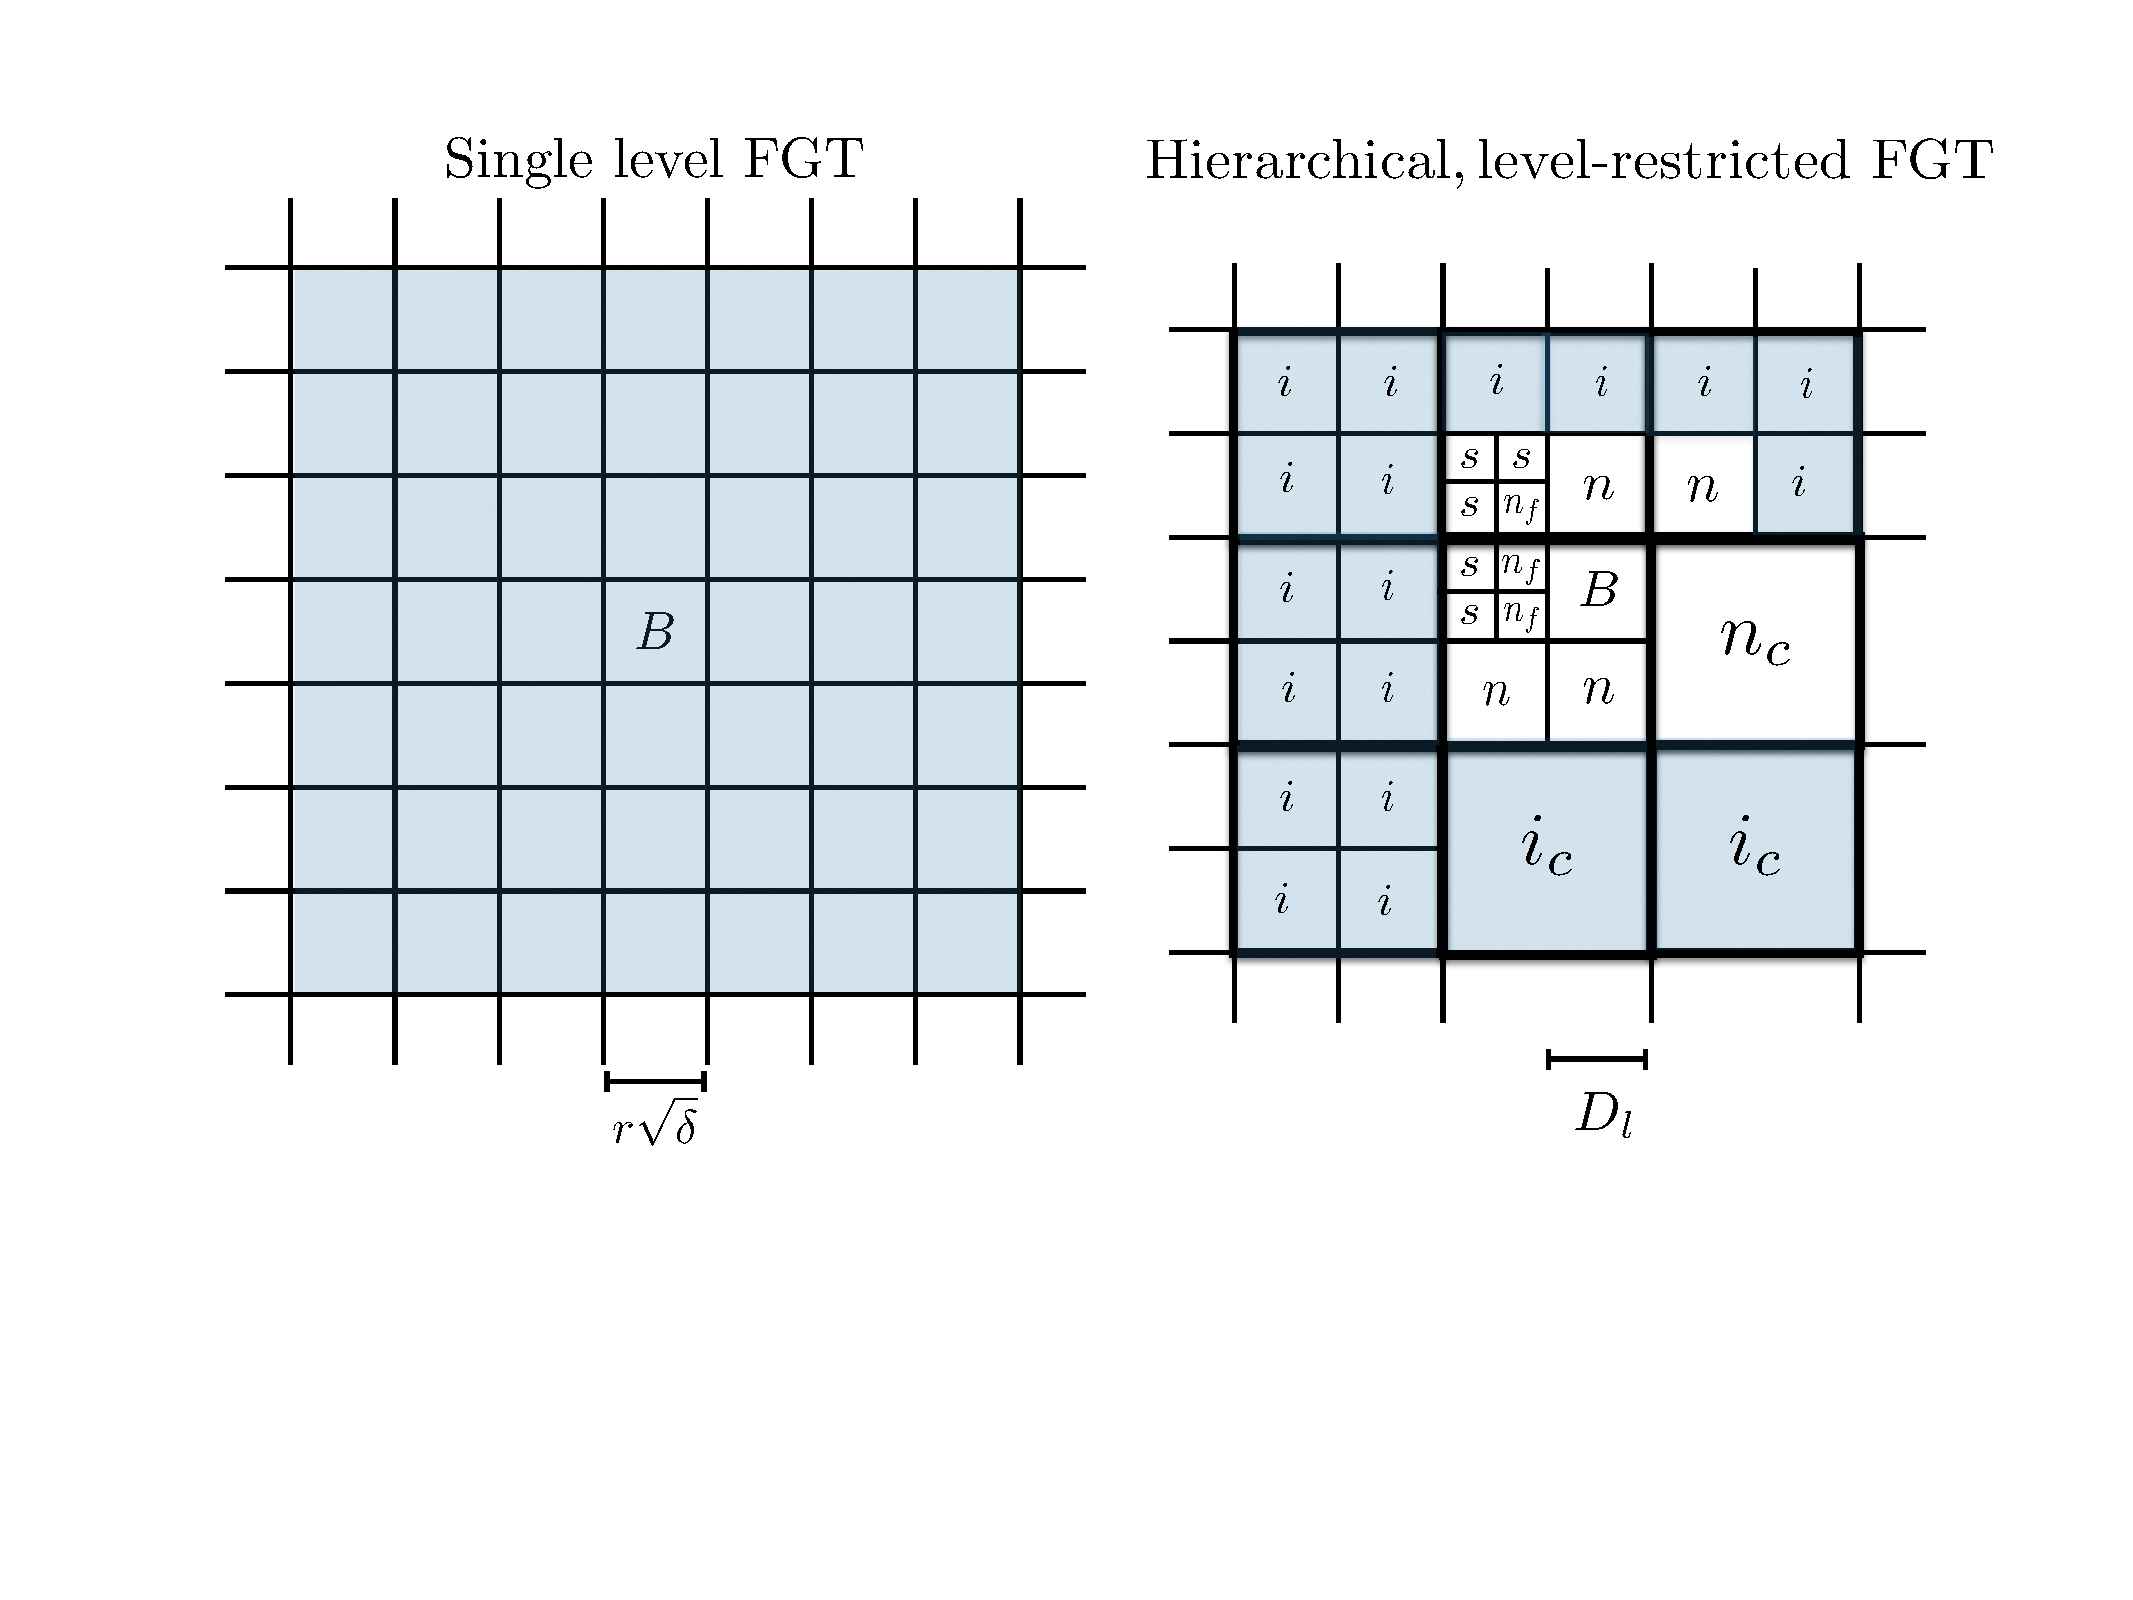
\includegraphics[height=0.68\textheight]{fgtadap.pdf}
\end{center}
\vspace{-0.5em}
\begin{center}
\footnotesize Adaptive FGT geometry. The output potential can require a
different adaptive tree from the input density.
\end{center}
\end{frame}

%================================================================
\begin{frame}{Systems of diffusion equations}
\small
For
\[
  \uvec_t=\mathbf{D}\Delta\uvec+\bm{F}(\uvec,\nabla\uvec,\x,t),
\]
where $\mathbf{D}=\diag(D_1,\ldots,D_m)$, each component has its own heat
kernel:
\[
  u_j(\x,t)=\Iop_{D_j}[u_{0,j}](\x,t)
  +\Vop_{D_j}[F_j](\x,t),
  \qquad j=1,\ldots,m.
\]

\begin{block}{Componentwise diffusion}
The diffusion part remains diagonal and exact. Coupling enters through the
reaction/advection term $\bm{F}$.
\end{block}
\end{frame}

%================================================================
\begin{frame}{Integral Adams methods}
\small
Let $t_n=n\dt$ and
\[
  \mathbf{U}(\uvec,\x,\tau)
  =
  \int_{\Omega}G(\x-\y,t_{n+1}-\tau)
  \bm{F}(\uvec(\y,\tau),\nabla\uvec(\y,\tau),\y,\tau)\dd\y.
\]
Then
\[
  \uvec_{n+1}(\x)=\Iop[\uvec_n](\x,\dt)
  +\int_{t_n}^{t_{n+1}}\mathbf{U}(\uvec,\x,\tau)\dd\tau.
\]
Approximate $\mathbf{U}$ in time by an interpolation polynomial and integrate:
\[
  \uvec_{n+1}(\x)=\Iop[\uvec_n](\x,\dt)
  +\dt\sum_{i=0}^s b_i
  \mathbf{U}_{n+1}(\uvec_{n+1-i},\x,t_{n+1-i}).
\]
\end{frame}

%================================================================
\begin{frame}{Adams coefficients}
\small
\begin{center}
\renewcommand{\arraystretch}{1.35}
\begin{tabular}{lll}
\toprule
Order & Adams--Moulton & Adams--Bashforth \\
\midrule
1 &
$b_0=1$ &
$b_1=1$ \\
2 &
$b_0=\frac12,\ b_1=\frac12$ &
$b_1=\frac32,\ b_2=-\frac12$ \\
4 &
$b_0=\frac9{24},\ b_1=\frac{19}{24},\
b_2=-\frac5{24},\ b_3=\frac1{24}$ &
$b_1=\frac{55}{24},\ b_2=-\frac{59}{24},\
b_3=\frac{37}{24},\ b_4=-\frac9{24}$ \\
\bottomrule
\end{tabular}
\end{center}

\begin{block}{Same coefficients, different objects}
The coefficients are classical Adams coefficients, but they multiply
heat-potential evaluations rather than pointwise right-hand sides.
\end{block}
\end{frame}

%================================================================
\begin{frame}{Delta-function property of the Green's function}
\small
For Adams--Moulton, $b_0\ne0$ and the term at $t_{n+1}$ appears.
Using the delta-function property of the Green's function,
\[
\begin{aligned}
\mathbf{U}_{n+1}(\uvec_{n+1},\x,t_{n+1})
&=\lim_{\tau\to t_{n+1}}
\int_{\Omega}G(\x-\y,t_{n+1}-\tau)
\bm{F}(\uvec(\y,\tau),\y,\tau)\dd\y \\
&=\bm{F}(\uvec_{n+1}(\x),\x,t_{n+1}).
\end{aligned}
\]

\begin{block}{Consequence}
For semilinear problems, the implicit term is pointwise in space.
\end{block}
\end{frame}

%================================================================
\begin{frame}{Semilinear implicit solve}
\small
For $\bm{F}=\bm{F}(\uvec,\x,t)$,
\[
  \uvec_{n+1}(\x)-\dt b_0
  \bm{F}(\uvec_{n+1}(\x),\x,t_{n+1})
  =\bm{g}(\x),
\]
where
\[
  \bm{g}(\x)=\Iop[\uvec_n](\x,\dt)
  +\dt\sum_{i=1}^{s-1}b_i
  \mathbf{U}_{n+1}(\uvec_{n+1-i},\x,t_{n+1-i}).
\]

\begin{itemize}
  \item Scalar problem: secant iteration at each target.
  \item System problem: small Newton solve at each target.
  \item No globally coupled nonlinear elliptic solve is created.
\end{itemize}
\end{frame}

%================================================================
\begin{frame}{State carried between heat-box steps}
\small
At time $t_n$, the semilinear solver stores $u_n$ and the propagated forcing
potentials
\[
  \mathcal H_j^n(\x)=
  \int_\Omega G(\x-\y,j\dt)
  F(u_{n-j}(\y),\y,t_{n-j})\dd\y,
  \qquad j=1,\ldots,s-2.
\]
These are exactly the stored history arrays in the Adams--Moulton code.

\begin{block}{Why this is sufficient}
The semigroup advances an old forcing contribution by one step through one
additional heat-potential evaluation. The complete time history is never
recomputed.
\end{block}
\end{frame}

%================================================================
\begin{frame}{One semilinear heat-box step}
\small
Given the adaptive tree and the state at $t_n$:
\begin{enumerate}
  \item Evaluate $\Iop_{\dt}[u_n]$ with the adaptive FGT.
  \item Advance the stored $\mathcal H_j^n$ by one heat step and form the
  known Adams right-hand side $\bm g$.
  \item At each Chebyshev node, solve the pointwise Adams--Moulton equation
  for $u_{n+1}$.
  \item Evaluate $F(u_{n+1},\x,t_{n+1})$, refine or coarsen the quadtree, and
  transfer $u_{n+1}$ and the stored history to the updated tree.
  \item Enforce the level-restriction condition.
\end{enumerate}

\begin{block}{Code structure}
The FGT, pointwise nonlinear solve, and adaptive-tree update are separate
components of every time step.
\end{block}
\end{frame}

%================================================================
\begin{frame}{Loss of locality in nonlinear coupling}
\small
If the forcing depends on gradients,
\[
  \bm{F}=\bm{F}(\uvec,\nabla\uvec,\x,t),
\]
then $\bm{F}(\uvec_{n+1},\nabla\uvec_{n+1})$ couples neighboring spatial points.

\begin{block}{Algorithmic choice}
For Navier--Stokes, use explicit or predictor-corrector treatment of the
advective term, while keeping diffusion in the heat-potential representation.
\end{block}

\[
  \text{implicit diffusion}
  \quad+\quad
  \text{explicit/predicted advection}
  \quad+\quad
  \text{projection}.
\]
\end{frame}

%================================================================
\begin{frame}{Heat example}
\small
\begin{center}
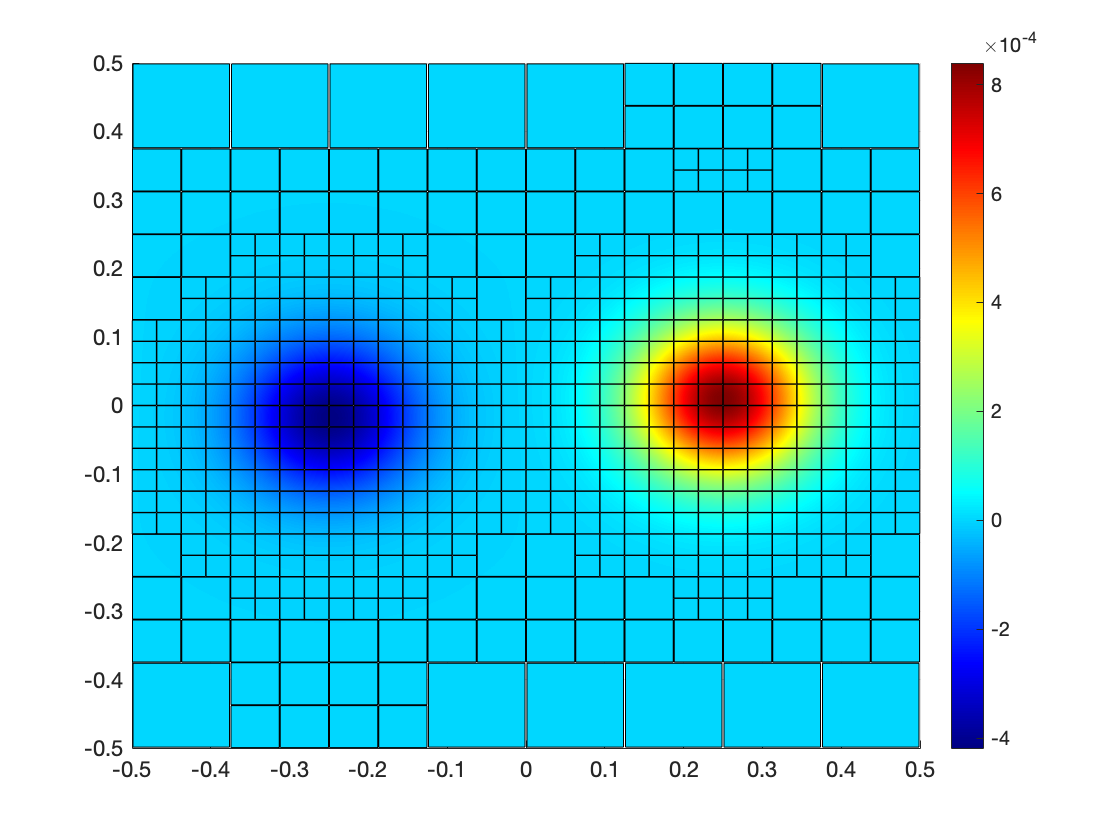
\includegraphics[width=0.31\textwidth]{heat_test3_t001_leaf592.png}
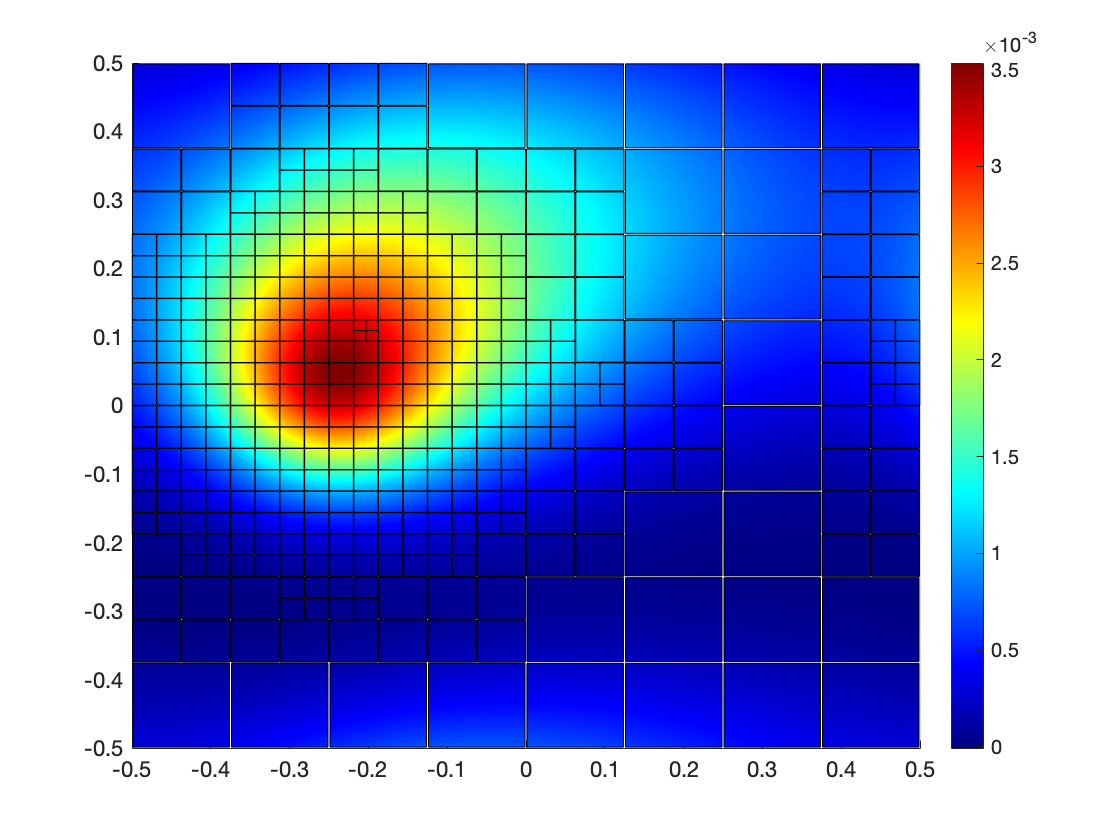
\includegraphics[width=0.31\textwidth]{heat_test3_t05_leaf409.png}
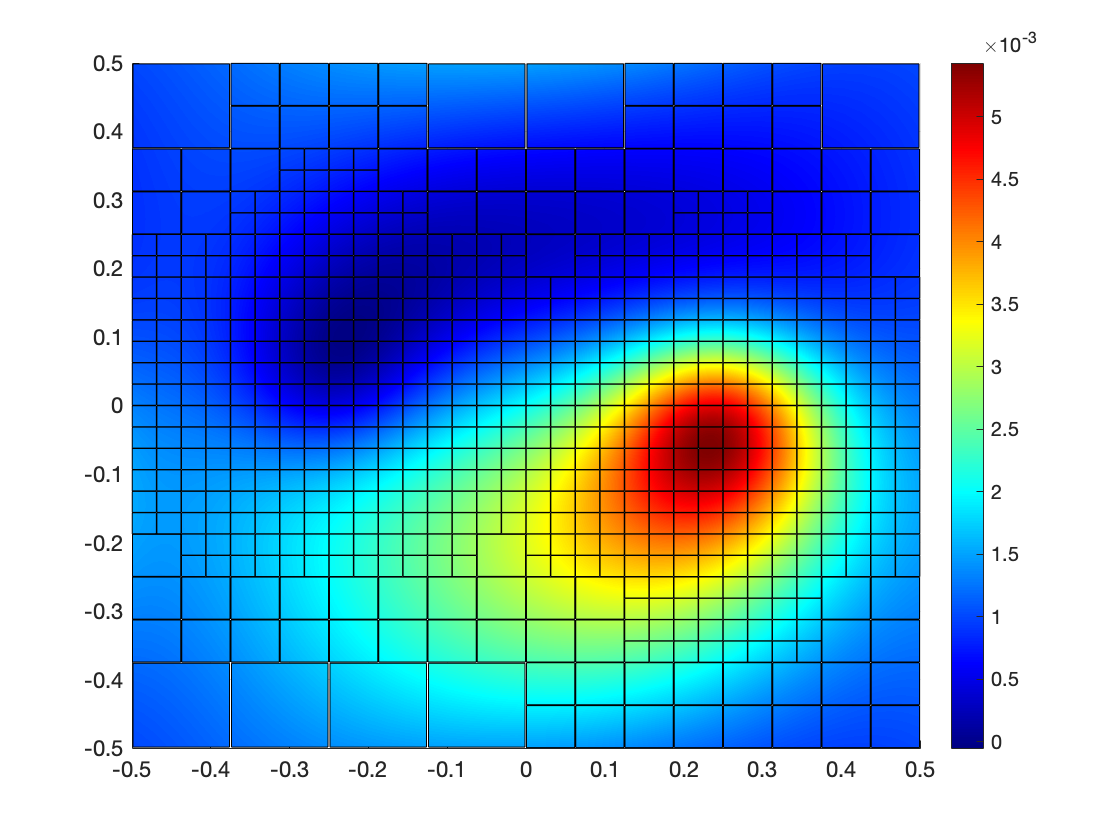
\includegraphics[width=0.31\textwidth]{heat_test3_t100_leaf652.png}
\end{center}
\vspace{-0.5em}
\begin{center}
\footnotesize Periodic heat equation at $t=0.001$, $0.05$, and $0.10$
(left to right), with $592$, $409$, and $652$ leaf boxes.
\end{center}

\end{frame}

%================================================================
\begin{frame}{Incompressibility in a periodic box}
\small
For a periodic vector field $\F$, write the Helmholtz decomposition
\[
  \F=\F_S+\F_G,\qquad
  \nabla\cdot\F_S=0,\qquad \F_G=\nabla\phi.
\]
In Fourier variables, for $\kvec\ne0$,
\[
  \widehat{\F_S}(\kvec)=
  \left(I-\frac{\kvec\kvec^T}{|\kvec|^2}\right)\widehat{\F}(\kvec),
  \qquad
  \widehat{\F_G}(\kvec)=
  \frac{\kvec\kvec^T}{|\kvec|^2}\widehat{\F}(\kvec).
\]

\begin{block}{Numerical operation}
On adaptive grids, evaluating this projection requires a fast Poisson/Laplace
potential calculation.
\end{block}
\end{frame}

%================================================================
\begin{frame}{Projection as a Poisson solve}
\small
The gradient part is
\[
  \F_G=\nabla\phi,\qquad \Delta\phi=\nabla\cdot\F.
\]
Then
\[
  \F_S=\F-\nabla\phi.
\]

\begin{block}{Periodic compatibility}
The zero Fourier mode is fixed by choosing $\phi$ to have mean zero.
Only the nonzero modes are inverted.
\end{block}

On adaptive point sets, this same operation is a Laplace volume-potential
evaluation plus differentiation, not a uniform-grid FFT-only operation.
\end{frame}

%================================================================
\begin{frame}{Unsteady Stokes in a periodic box}
\small
The linearized incompressible equations are
\[
  \uvec_t=\nu\Delta\uvec-\nabla p+\F(\x,t),
  \qquad
  \nabla\cdot\uvec=0.
\]
Decompose
\[
  \F=\F_S+\F_G,\qquad \F_G=\nabla\phi.
\]
Then
\[
  \uvec(\x,t)=\Iop[\uvec_0](\x,t)+\Vop[\F_S](\x,t),
  \qquad
  \nabla p(\x,t)=\F_G(\x,t).
\]

\begin{block}{Helmholtz decomposition consequence}
Only the solenoidal forcing drives the velocity. The gradient part becomes
pressure.
\end{block}
\end{frame}

%================================================================
\begin{frame}{Stokes algorithmic pipeline}
\small
For each time step:
\begin{enumerate}
  \item Given $\F(\cdot,t_m)$ at required Adams nodes, compute $\F_S$ by
  Helmholtz projection.
  \item Evaluate heat potentials involving $\uvec_n$ and the projected
  forcing history on the current slab.
  \item Adapt the tree to resolve $\uvec_{n+1}$ and any required projected
  forcing values.
  \item Recover pressure gradient from $\F_G$ if needed.
\end{enumerate}

\begin{block}{Fast work}
Heat potentials use the FGT; projection uses Poisson/Laplace fast solvers.
\end{block}
\end{frame}

%================================================================
\begin{frame}{Unsteady Stokes example}
\small
\begin{center}
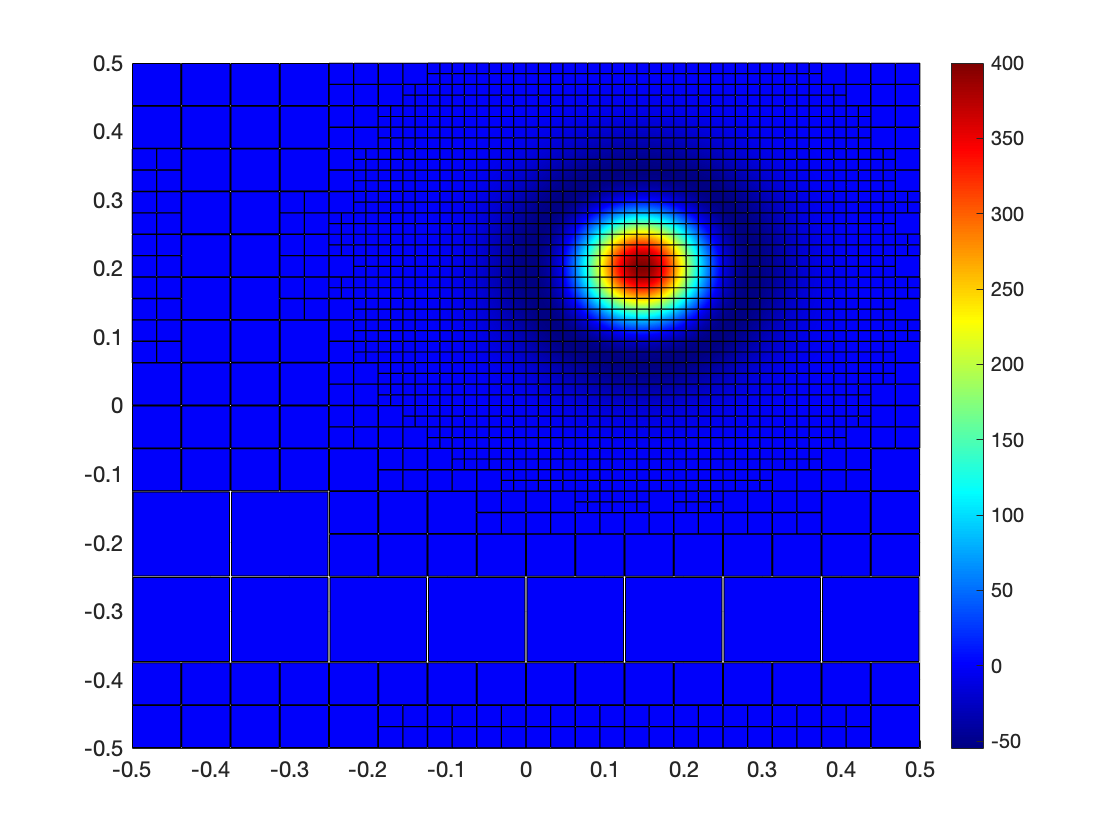
\includegraphics[width=0.31\textwidth]{t10_1882.png}
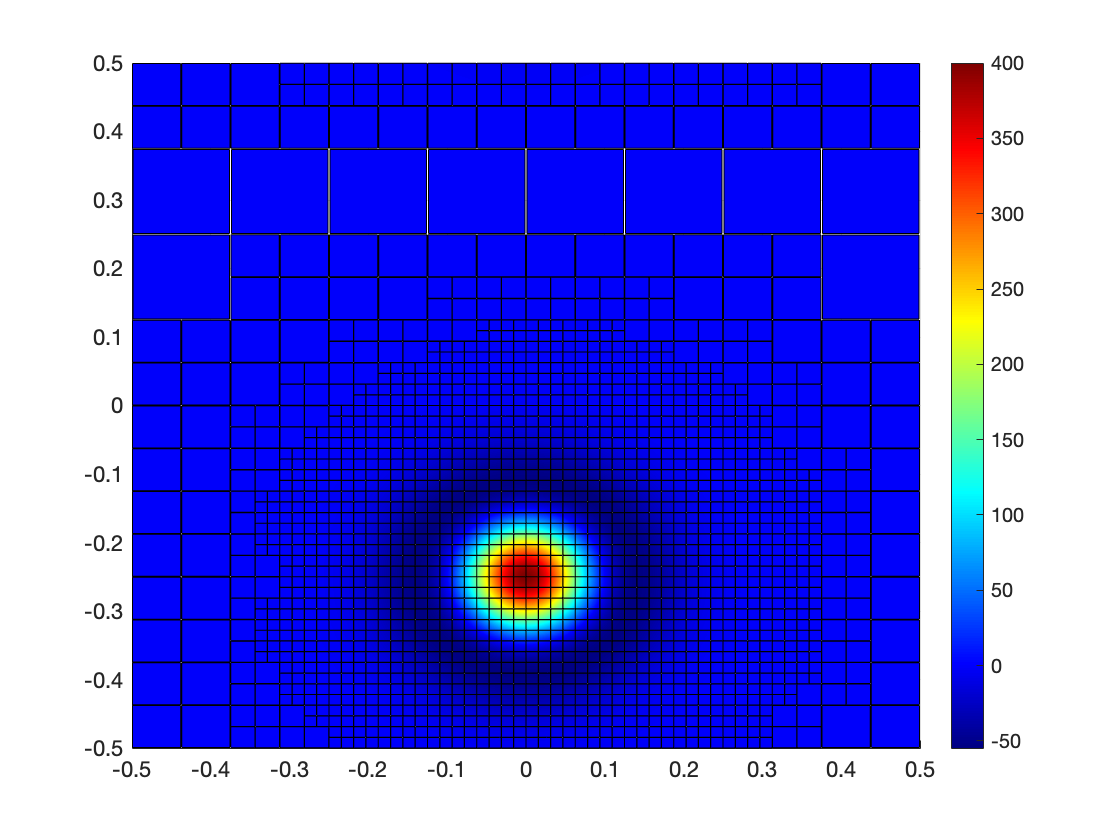
\includegraphics[width=0.31\textwidth]{t50_1854.png}
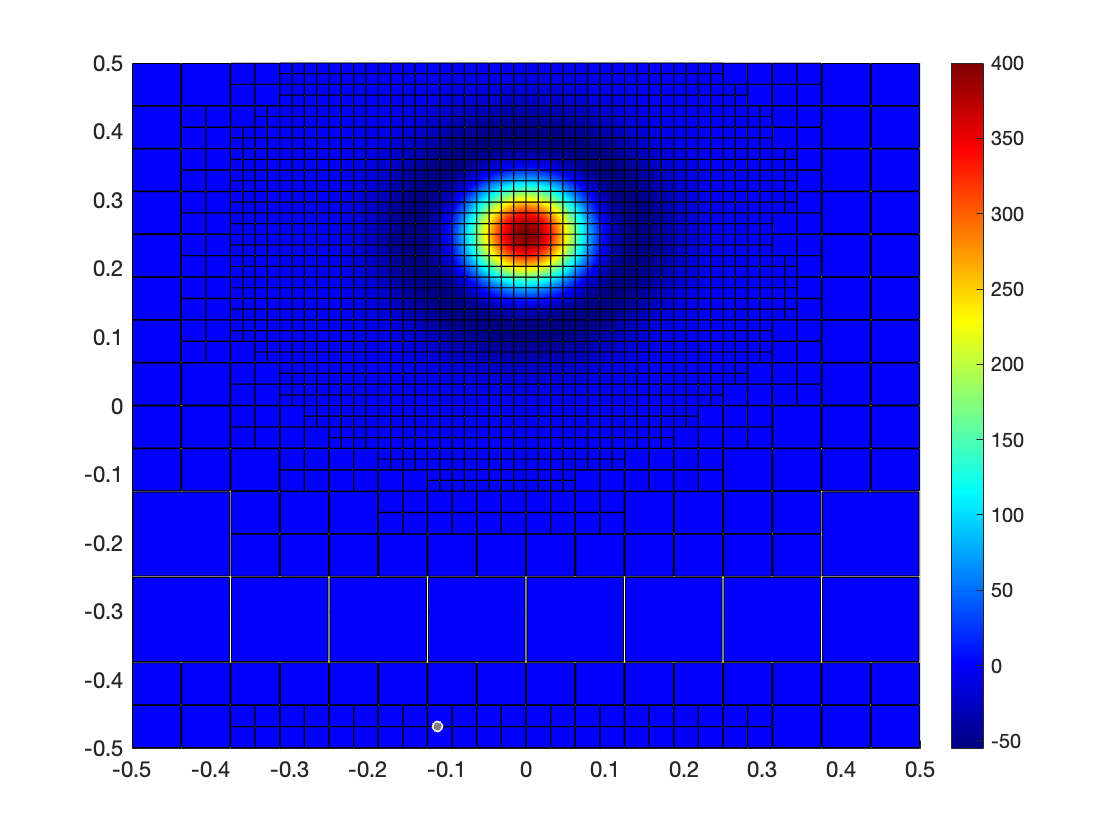
\includegraphics[width=0.31\textwidth]{t100_1804.png}
\end{center}
\vspace{-0.5em}
\begin{center}
\footnotesize Unsteady Stokes vorticity at $t=0.01$, $0.05$, and $0.10$
(left to right), with $1882$, $1854$, and $1804$ leaf boxes.
\end{center}
\end{frame}

%================================================================
\begin{frame}{Navier--Stokes as a Volterra equation}
\small
In a periodic box,
\[
  \uvec_t=\nu\Delta\uvec-\nabla p-(\uvec\cdot\nabla)\uvec+\f,
  \qquad \nabla\cdot\uvec=0.
\]
Define
\[
  \F(\uvec,\x,t)=-(\uvec\cdot\nabla)\uvec+\f(\x,t),
  \qquad
  \F=\F_S+\F_G.
\]
Then
\[
  \uvec(\x,t)=\Iop[\uvec_0](\x,t)+\Vop[\F_S,\uvec](\x,t).
\]

\begin{block}{Volterra form}
The incompressible Navier--Stokes PDE becomes a nonlinear Volterra integral
equation with heat smoothing and Helmholtz projection.
\end{block}
\end{frame}

%================================================================
\begin{frame}{Predictor-corrector for Navier--Stokes}
\small
For order $s$:
\begin{enumerate}
  \item Predict $\uvec_{n+1}^p$ with an Adams--Bashforth heat-potential formula.
  \item Evaluate
  \[
    \F^p_{n+1}=-(\uvec^p_{n+1}\cdot\nabla)\uvec^p_{n+1}
    +\f_{n+1}.
  \]
  \item Project $\F^p_{n+1}$ to obtain $(\F^p_{n+1})_S$.
  \item Correct with the Adams--Moulton formula using the predicted forcing.
\end{enumerate}

\begin{block}{Predictor-corrector role}
It improves the stability region for advection while preserving the
heat-potential treatment of diffusion.
\end{block}
\end{frame}

%================================================================
\begin{frame}{Advection still controls time step}
\small
The heat-potential method removes the parabolic restriction
\[
  \dt=\Oh(h^2/\nu)
\]
for the diffusive part. It does not remove all restrictions.

\begin{itemize}
  \item Explicit advection still imposes a convective scale
  $\dt\lesssim h/\|\uvec\|$.
  \item Nonlinear accuracy still requires resolving changes in time.
  \item Adaptive meshes make the smallest local $h$ important for explicit
  gradient-dependent terms.
\end{itemize}

\begin{block}{Stability interpretation}
The method removes the diffusive stability restriction; the remaining time-step
constraints come from nonlinear or advective effects.
\end{block}
\end{frame}

%================================================================
\begin{frame}{Double shear layer test}
\small
We use the classical double shear layer initial data
\[
  u_1(x,y,0)=
  \begin{cases}
  \tanh(\rho(y+0.25)), & x\le0,\\
  \tanh(\rho(-y+0.25)), & x>0,
  \end{cases}
\]
\[
  u_2(x,y,0)=\delta\sin(2\pi x),
  \qquad \delta=0.05,\quad \rho=30.
\]

\begin{block}{Test problem value}
Thin shear layers roll up into vortical structures, so the grid must refine
and coarsen dynamically.
\end{block}
\end{frame}

%================================================================
\begin{frame}{Navier--Stokes adaptive snapshots}
\small
\begin{center}
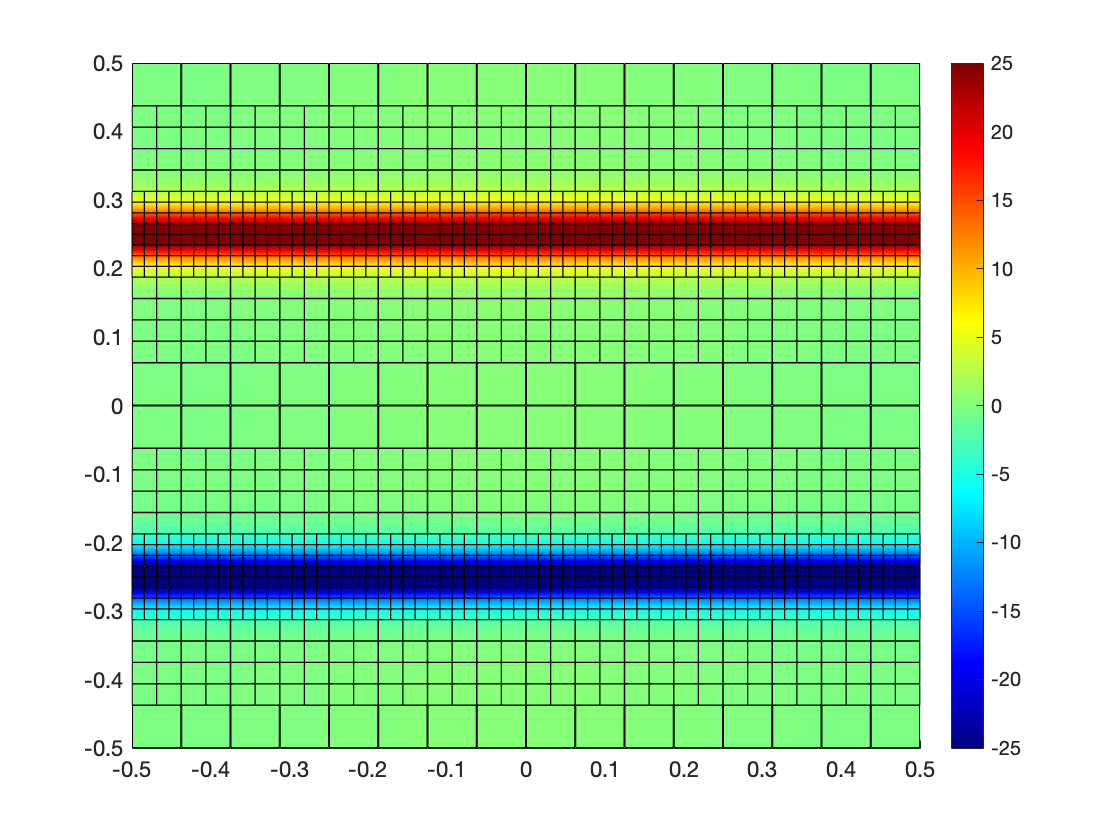
\includegraphics[width=0.31\textwidth]{t1_leaf1600.png}
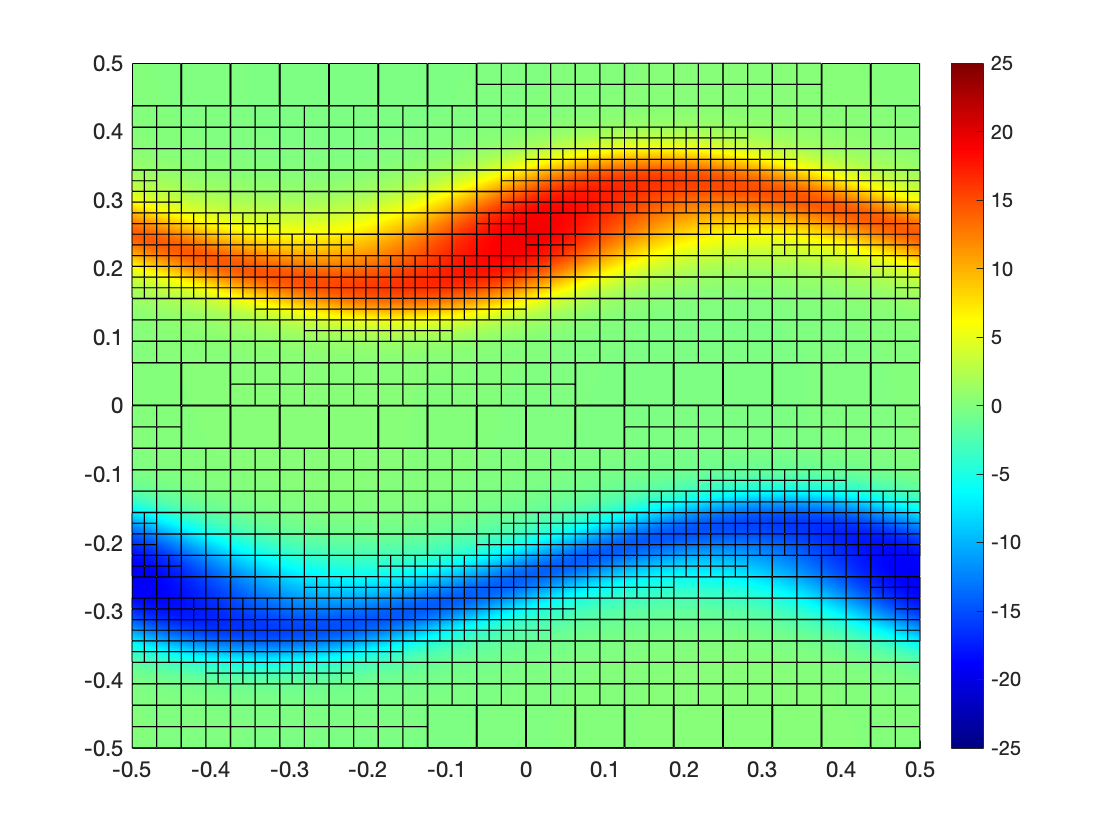
\includegraphics[width=0.31\textwidth]{t60_leaf1768.png}
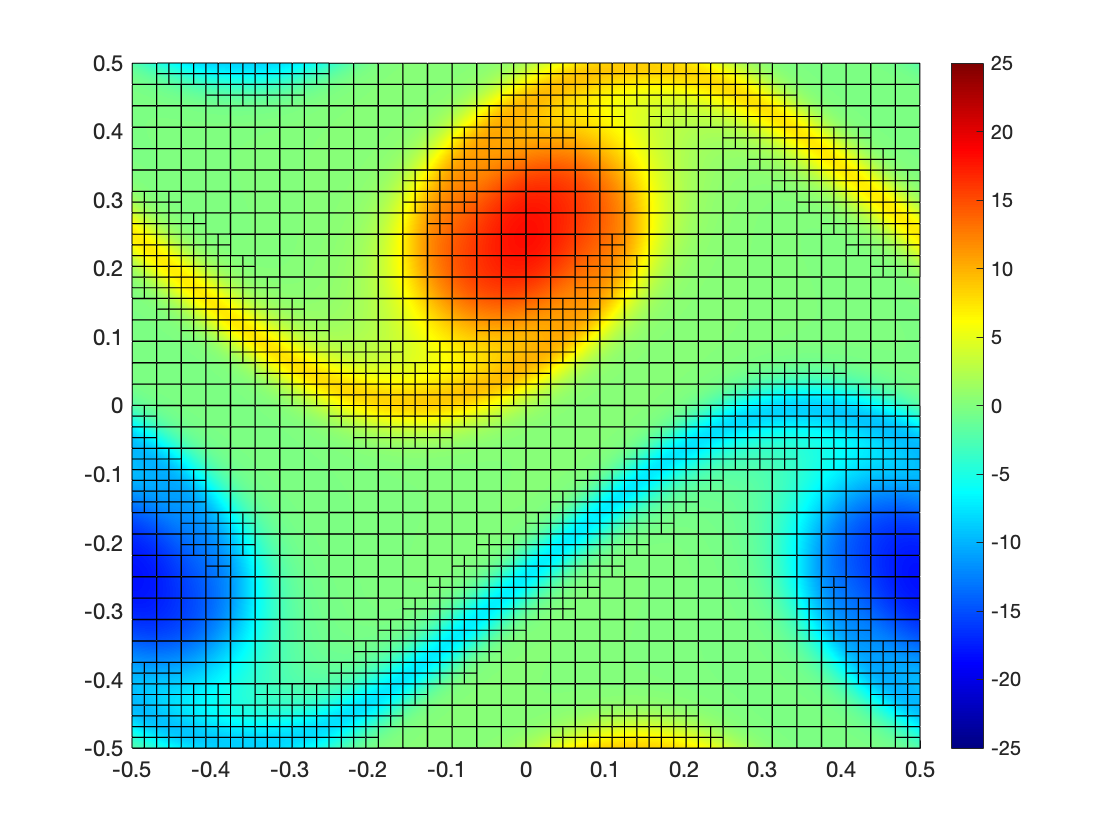
\includegraphics[width=0.31\textwidth]{t100_leaf2152.png}
\end{center}
\vspace{-0.5em}
\begin{center}
\footnotesize Double-shear-layer vorticity at $t=0.008$, $0.60$, and $1.20$
(left to right), each overlaid with the adaptive quadtree.
\end{center}
\end{frame}

%================================================================
\begin{frame}{Periodic heat and flow summary}
\small
\begin{itemize}
  \item Duhamel plus the heat semigroup gives a genuine time-marching method.
  \item High-order Adams formulas can be written directly for heat potentials.
  \item Semilinear implicit steps are pointwise nonlinear solves.
  \item Incompressibility is enforced by projecting the forcing before heat
  evolution.
  \item Adaptive grids are effective because potential evaluation can target
  newly created nodes accurately and quickly.
\end{itemize}

\end{frame}

%================================================================
\begin{frame}{Break}
\centering
\Large 10 minute break
\end{frame}

%================================================================
\section{SKIE Mode Calculation}

\begin{frame}{Mode calculation of optical waveguides}
\small
This section follows J. Lai and S. Jiang, ``Second kind integral equation
formulation for the mode calculation of optical waveguides,'' \emph{Applied
and Computational Harmonic Analysis}, 44(3) (2018), 645--664.

\begin{itemize}
  \item Photonic devices use straight waveguides as input and output channels.
  \item A waveguide supports a finite set of propagating modes determined by
  its geometry, wavelength, and refractive indices.
  \item The first step in a photonic simulation is to compute these modes
  accurately and efficiently.
\end{itemize}

\begin{block}{Sequence of the construction}
Mode ansatz $\longrightarrow$ two-dimensional layer potentials
$\longrightarrow$ four interface equations $\longrightarrow$ nonlinear
effective-index root finding.
\end{block}
\end{frame}

%================================================================
\begin{frame}{A typical photonic device}
\begin{columns}[c,totalwidth=\textwidth]
\begin{column}{0.47\textwidth}
\centering
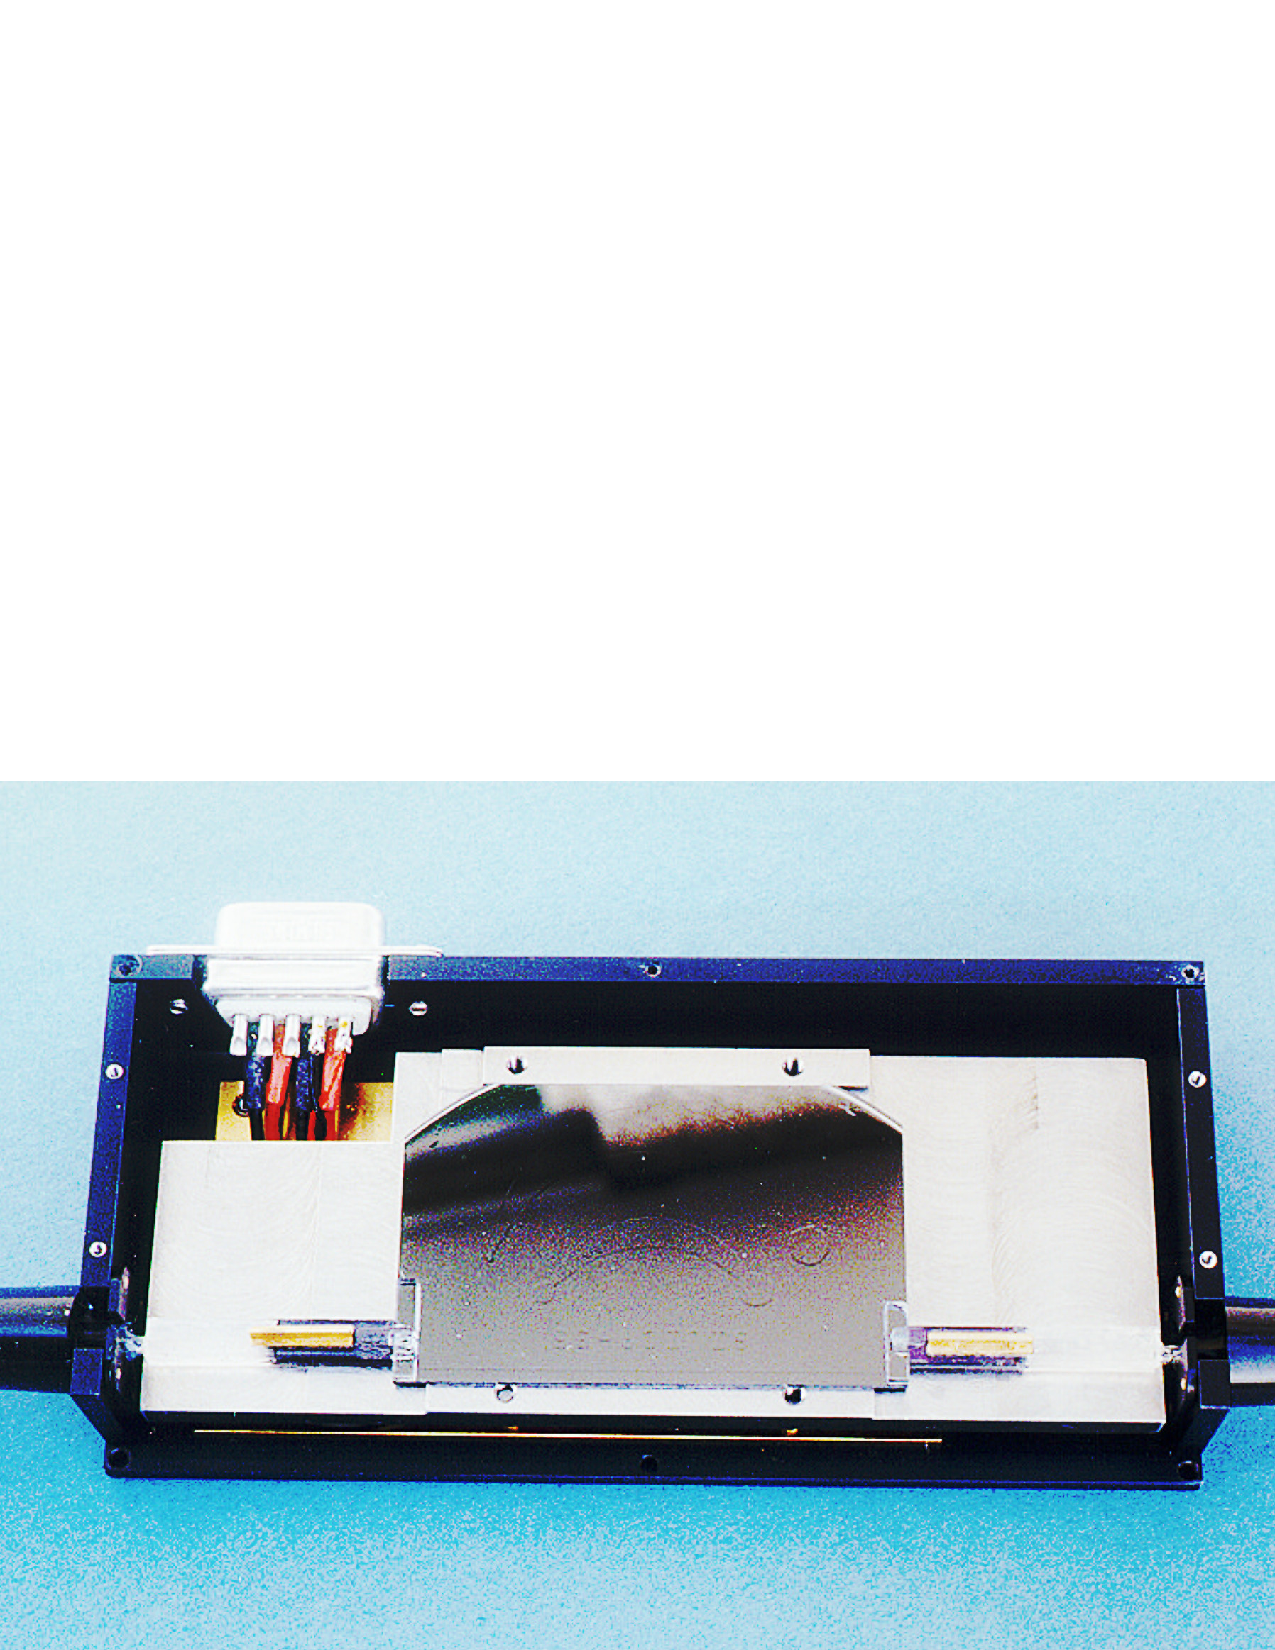
\includegraphics[width=\linewidth,height=0.62\textheight,keepaspectratio]{awg-package.pdf}\\[-0.35em]
\footnotesize Packaged arrayed waveguide grating module
\end{column}
\begin{column}{0.49\textwidth}
\centering
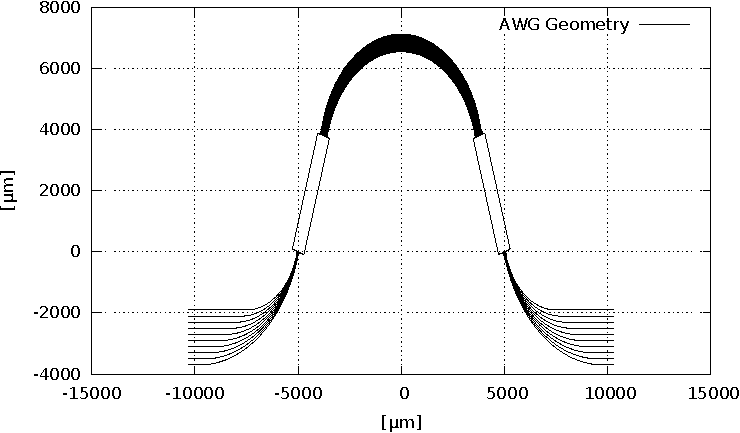
\includegraphics[width=\linewidth,height=0.62\textheight,keepaspectratio]{awg-crop.pdf}\\[-0.35em]
\footnotesize Plane geometry of an arrayed waveguide grating
\end{column}
\end{columns}
\end{frame}

%================================================================
\begin{frame}{Cross section of an optical waveguide}
\small
\begin{center}
\includegraphics[height=0.62\textheight]{illustration-eps-converted-to.pdf}
\end{center}

The cross section in the $xy$-plane can contain multiple cores with distinct
refractive indices. The electromagnetic fields propagate in the $z$ direction.
\end{frame}

%================================================================
\begin{frame}{Why use interface integral equations?}
\small
\begin{itemize}
  \item Finite-difference and finite-element methods discretize a truncated
  cross-section and impose artificial boundary or PML conditions.
  \item Multipole methods require circular, well-separated cores.
  \item Earlier BIE formulations can contain first-kind, hypersingular, or
  tangential-derivative terms.
\end{itemize}

\begin{block}{SKIE formulation objective}
Use unknown densities only on material interfaces and obtain a well-conditioned
second-kind system. The layer potentials satisfy Maxwell's equations in each
material region automatically.
\end{block}
\end{frame}

%================================================================
\begin{frame}{Maxwell equations and mode ansatz}
\small
With time dependence $e^{-\ii\omega t}$, rescale the magnetic field as in the
paper. In a material with $k=k_vn$,
\[
  \nabla\times\E-\ii k_v\Hfield=0,
  \qquad
  \nabla\times\Hfield+\ii\frac{k^2}{k_v}\E=0.
\]
For a waveguide mode, write the $z$ dependence as
\[
  \E(x,y,z)=\E(x,y)e^{\ii\beta z},
  \qquad
  \Hfield(x,y,z)=\Hfield(x,y)e^{\ii\beta z}.
\]
Here $\beta$ is the propagation constant.

If $k=k_v n$ in a material region, each scalar component satisfies
\[
  \left[\Delta_\perp+(k^2-\beta^2)\right]u=0.
\]
Equivalently,
\[
  k_{\beta}= \sqrt{k^2-\beta^2}.
\]
\end{frame}

%================================================================
\begin{frame}{Effective index}
\small
Let
\[
  k_v=\frac{\omega}{c},\qquad k_j=k_v n_j,
  \qquad n_e=\frac{\beta}{k_v}.
\]
Then in material region $j$,
\[
  k_{\beta,j}=k_v\sqrt{n_j^2-n_e^2}.
\]

\vspace{2mm}
The effective index $n_e$ is the nonlinear spectral parameter.
\end{frame}

%================================================================
\begin{frame}{Why the imaginary part of $n_e$ matters}
\small
The modal confinement loss in dB/m is
\[
  L=\frac{20}{\ln(10)}\,\frac{2\pi}{\lambda}\,Im(n_e)\,10^9,
\]
where $\lambda$ is the vacuum wavelength in nanometers.

\begin{itemize}
  \item The real part of $n_e$ governs phase propagation.
  \item The imaginary part governs attenuation and can be many orders of
  magnitude smaller than the real part.
  \item Accurate mode calculation must therefore resolve both components of
  the effective index.
\end{itemize}
\end{frame}

%================================================================
\begin{frame}{Interface boundary conditions}
\small
Across a material interface, tangential electromagnetic fields are continuous:
\[
  [\nvec\times\E]=0,\qquad [\nvec\times\Hfield]=0.
\]
For a waveguide interface, the two tangential directions are $z$ and
the cross-section tangent $\tvec$. Thus
\[
  [E_z]=0,\qquad [E_\tau]=0,\qquad
  [H_z]=0,\qquad [H_\tau]=0.
\]

\begin{block}{Four scalar conditions}
The SKIE formulation uses four interface densities, matching the four
tangential continuity conditions.
\end{block}
\end{frame}

%================================================================
\begin{frame}{Longitudinal components determine the fields}
\small
For a mode, the transverse components are determined by $E_z$ and $H_z$.
One such form is
\[
\begin{bmatrix}H_x\\ E_y\end{bmatrix}
=
\frac{-1}{k^2-\beta^2}
\begin{bmatrix}
\ii k^2/k_v & -\ii\beta\\
-\ii\beta & \ii k_v
\end{bmatrix}
\begin{bmatrix}
\partial_y E_z\\ \partial_x H_z
\end{bmatrix},
\]
\[
\begin{bmatrix}E_x\\ H_y\end{bmatrix}
=
\frac{1}{k^2-\beta^2}
\begin{bmatrix}
\ii\beta & \ii k_v\\
\ii k^2/k_v & \ii\beta
\end{bmatrix}
\begin{bmatrix}
\partial_x E_z\\ \partial_y H_z
\end{bmatrix}.
\]
\end{frame}

%================================================================
\begin{frame}{Need for transverse-field consistency}
\small
Representations based only on $E_z,H_z$ can contain:
\begin{itemize}
  \item hypersingular operators;
  \item tangential derivatives of unknown densities;
  \item first-kind blocks;
\end{itemize}

\begin{block}{SKIE design}
Start from a vector electromagnetic representation and combine single and
double layer terms so the hypersingular parts cancel.
\end{block}
\end{frame}

%================================================================
\begin{frame}{3D-to-2D layer reduction}
\small
A scalar 3D Helmholtz single layer on an infinite cylinder has kernel
\[
  \frac{e^{\ii k|\bm r-\bm r'|}}{4\pi|\bm r-\bm r'|}.
\]
With density
\[
  \sigma(x,y,z)=\mu(x,y)e^{\ii\beta z},
\]
Sommerfeld's identity gives
\[
  \int_{-\infty}^{\infty}
  \frac{e^{\ii k\sqrt{a^2+t^2}}}{4\pi\sqrt{a^2+t^2}}
  e^{-\ii\beta t}\dd t
  =
  \frac{\ii}{4}H_0^{(1)}(k_\beta a).
\]
Thus the 3D layer reduces to a 2D Helmholtz single layer.
\end{frame}

%================================================================
\begin{frame}{2D Helmholtz layer operators}
\small
For a boundary $\Gamma$,
\[
  \Sop[\sigma](P)=\int_\Gamma
  \frac{\ii}{4}H_0^{(1)}(k_\beta|P-Q|)
  \sigma(Q)\dd s_Q.
\]
The double layer and normal derivative operators are
\[
  \Dop[\sigma](P)=\int_\Gamma
  \partial_{\nu(Q)}G_\beta(P,Q)\sigma(Q)\dd s_Q,
\]
\[
  \Sop_\nu[\sigma](P)=\partial_{\nu(P)}\Sop[\sigma](P),
  \qquad
  \Sop_\tau[\sigma](P)=\partial_{\tau(P)}\Sop[\sigma](P).
\]
The SKIE also uses
\[
  \Top[\sigma](P)=\int_\Gamma
  \partial_{\tau(Q)}G_\beta(P,Q)\sigma(Q)\dd s_Q.
\]
\end{frame}

%================================================================
\begin{frame}{Layer fields from densities}
\small
After the 3D-to-2D reduction, in a material with refractive index $n$, the
nondimensionalized longitudinal components are
\[
\begin{aligned}
\widetilde H_z
&=n^2\Dop[J_\tau]
  +n_e\Top[M_\tau]
  +\ii(n^2-n_e^2)\Sop[M_z],\\
\widetilde E_z
&=-n_e\Top[J_\tau]
  -\ii(n^2-n_e^2)\Sop[J_z]
  +\Dop[M_\tau].
\end{aligned}
\]

\begin{block}{Consequence for assembly}
Substituting these traces into the four continuity conditions produces the
block SKIE system.
\end{block}
\end{frame}

\begin{frame}{Four surface/interface densities}
\small
The unknown vector is
\[
  x=
  \begin{bmatrix}
  J_\tau\\ J_z\\ M_\tau\\ M_z
  \end{bmatrix}.
\]
Here $\J$ and $\M$ are electric and magnetic surface-current-type densities
restricted to the material interface:
\[
  \J=J_\tau\tvec+J_z\hat{\bm z},
  \qquad
  \M=M_\tau\tvec+M_z\hat{\bm z}.
\]

\begin{block}{Interface-only discretization}
If there are $N$ boundary nodes, the matrix size is $4N\times4N$ for one
interface, and block-structured for many interfaces.
\end{block}
\end{frame}

%================================================================
\begin{frame}{SKIE formulation for mode calculation}
\scriptsize
For two materials with refractive indices $n_0,n_1$, the boundary
conditions lead to
\[
  (D+A(n_e))x=0,
  \qquad x=(J_\tau,J_z,M_\tau,M_z)^T,
\]
where
\[
  D=\diag\left(
  \frac{n_0^2+n_1^2}{2},
  \frac{n_0^2+n_1^2}{2},
  1,
  1
  \right),
\]
and the compact block has the structure
\[
A(n_e)=\begin{bmatrix}
A_{11}&0&A_{13}&A_{14}\\
A_{21}&A_{22}&A_{23}&A_{24}\\
-A_{13}&-A_{14}&A_{33}&0\\
-A_{23}&-A_{24}&A_{43}&A_{44}
\end{bmatrix}.
\]
For a $C^2$ interface, all entries of $A(n_e)$ are compact.

\begin{block}{Mode condition}
The effective index $n_e$ is an electromagnetic mode when this homogeneous
system has a nontrivial null vector.
\end{block}
\end{frame}

\begin{frame}{Nonlinear eigenvalue problem}
\small
After discretization,
\[
  M(n_e)x=0.
\]
The matrix depends nonlinearly on $n_e$ through
\[
  k_{\beta,j}=k_v\sqrt{n_j^2-n_e^2}
\]
inside every layer kernel.

We locate roots through a scalar analytic function derived from
$M(n_e)^{-1}$, then compute the associated null vector.
\end{frame}

%================================================================
\begin{frame}{Muller root function}
\small
We use a scalar analytic root function of the form
\[
  f(n_e)=\frac{1}{u^T M(n_e)^{-1}v},
\]
where $u$ and $v$ are fixed random vectors.

Muller's method is applied to find a zero of $f(n_e)$; the corresponding
matrix $M(n_e)$ has a nontrivial null vector.

\end{frame}

%================================================================
\begin{frame}{Discretization of interfaces}
\small
For smooth curves:
\begin{itemize}
  \item split each interface into chunks of equal parameter length;
  \item use shifted and scaled $p$-point Gauss--Legendre nodes on each chunk;
  \item use generalized Gaussian quadrature for same-chunk interactions;
  \item use adaptive Gaussian integration for interactions between distinct
  chunks.
\end{itemize}

For corners:
\begin{itemize}
  \item use dyadically refined chunks toward each corner;
  \item the same layer-potential construction is used on the refined mesh.
\end{itemize}
\end{frame}

%================================================================
\begin{frame}{Many-interface assembly}
\small
For photonic crystal fibers or multi-core waveguides, there are interfaces
\[
  \Gamma=\Gamma_1\cup\cdots\cup\Gamma_m.
\]
The unknown vector becomes
\[
  x=(x_1,\ldots,x_m),\qquad
  x_\ell=(J_{\tau,\ell},J_{z,\ell},M_{\tau,\ell},M_{z,\ell}).
\]

\begin{block}{Block structure}
Diagonal blocks contain self-interface singular quadrature. Off-diagonal
blocks are smooth interactions between distinct interfaces and are easier
to evaluate or accelerate.
\end{block}
\end{frame}

%================================================================
\begin{frame}{SKIE algorithm}
\small
For a fixed frequency:
\begin{enumerate}
  \item Choose a search window for $n_e$ using material indices and physical
  expectations.
  \item For each trial $n_e$, assemble or apply $M(n_e)=D+A(n_e)$ through the
  transverse wavenumbers $k_{\beta,j}$.
  \item Evaluate the scalar root function $f(n_e)$.
  \item Refine a root with Muller's method.
  \item Compute the null vector $x$ and reconstruct fields.
\end{enumerate}
\end{frame}

%================================================================
\begin{frame}{Rectangular waveguide benchmark}
\small
We consider the high-index-contrast silica waveguide used in the SKIE paper:
\begin{itemize}
  \item square cross section with side length $3.4\,\mu\mathrm m$;
  \item cladding index $n_0=1.4447$;
  \item core index $n_1=1.4447\times1.02$;
  \item incident wavelength $1550\,\mathrm{nm}$.
\end{itemize}

This waveguide has one propagation constant with double degeneracy. Its
effective index is approximately $1.458\ldots$.
\end{frame}

%================================================================
\begin{frame}{Layered rectangular waveguide geometry}
\begin{center}
\includegraphics[height=0.70\textheight]{waveguide2-eps-converted-to.pdf}
\end{center}
\begin{center}
\footnotesize General cross-sectional notation for a layered rectangular
waveguide. The numerical benchmark specializes this setting.
\end{center}
\end{frame}

%================================================================
\begin{frame}{Rectangular waveguide: GMRES iterations under refinement}
\small
For the rectangular-waveguide conditioning test at $n_e=1.451$, we obtain the
following GMRES iteration counts:
\begin{center}
\large
\renewcommand{\arraystretch}{1.45}
\[
\begin{array}{c|ccccc}
\text{points per side} & 150 & 300 & 450 & 600 & 750\\
\hline
\text{GMRES iterations} & 32 & 32 & 32 & 34 & 34
\end{array}
\]
\end{center}

In this test, refinement from $150$ to $750$ points per side changes the
iteration count only from $32$ to $34$.
\end{frame}

%================================================================
\begin{frame}{Effective-index convergence: SKIE versus SREP}
\scriptsize
For the same $3.4\,\mu\mathrm m$ square silica waveguide at wavelength
$1550\,\mathrm{nm}$, we obtain:
\begin{center}
\renewcommand{\arraystretch}{1.25}
\begin{tabular}{c|cc|cc}
\toprule
& \multicolumn{2}{c|}{SREP} & \multicolumn{2}{c}{SKIE}\\
$N$ & $\Re n_e$ & $\Im n_e$ & $\Re n_e$ & $\Im n_e$\\
\midrule
150 & 1.45867110663907 & $3\times10^{-10}$ &
1.45860141500175 & $3\times10^{-9}$\\
300 & 1.45884317112249 & $-2\times10^{-10}$ &
1.45860141488787 & $6\times10^{-11}$\\
450 & 1.45890000315967 & $9\times10^{-14}$ &
1.45860141488572 & $1\times10^{-12}$\\
600 & 1.45887005720651 & $-7\times10^{-6}$ &
1.45860141488567 & $3\times10^{-14}$\\
\bottomrule
\end{tabular}
\end{center}

\begin{block}{Observed behavior}
The SKIE values converge consistently to about 13 digits, while the
single-layer representation (SREP) is erratic as the discretization is refined.
\end{block}
\end{frame}

%================================================================
\begin{frame}{Complex waveguide geometries}
\small
\begin{columns}[c,totalwidth=\textwidth]
\begin{column}{0.48\textwidth}
\centering
\includegraphics[height=0.58\textheight]{ring120-eps-converted-to.pdf}\\[-0.3em]
\footnotesize Photonic crystal fiber with 121 holes
\end{column}
\begin{column}{0.48\textwidth}
\centering
\includegraphics[height=0.58\textheight]{ring48-eps-converted-to.pdf}\\[-0.3em]
\footnotesize Photonic crystal fiber with 48 holes
\end{column}
\end{columns}

\begin{center}
\footnotesize Interface unknowns allow the same SKIE construction for both
multi-core and multi-hole cross sections.
\end{center}
\end{frame}

%================================================================
\begin{frame}{PCF effective-index accuracy: hexagon ring}
\small
\begin{center}
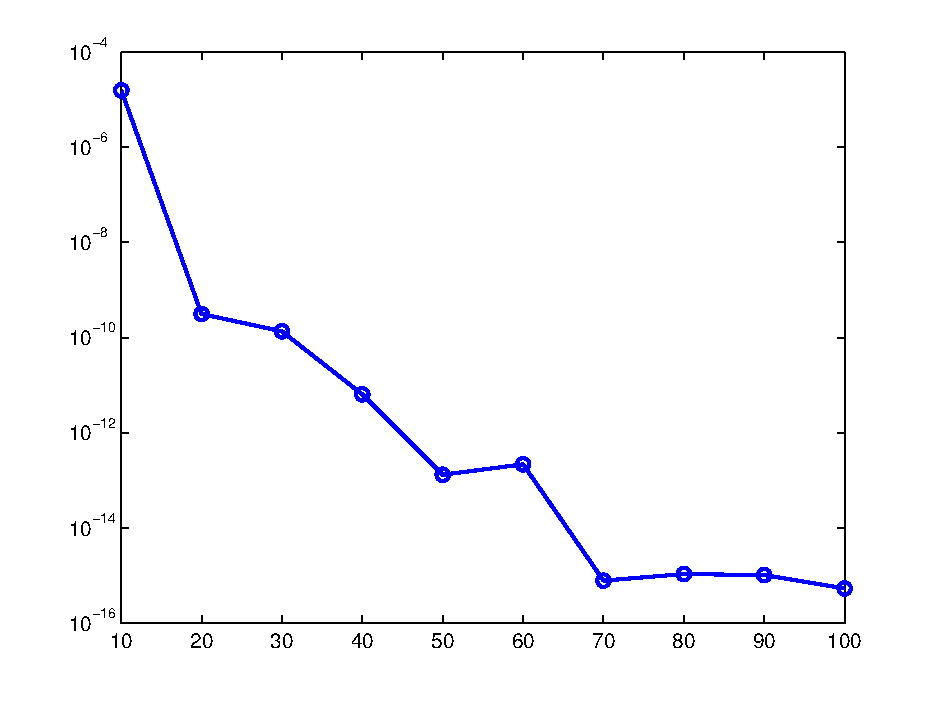
\includegraphics[height=0.74\textheight]{convergence2_cropped.pdf}
\end{center}
\vspace{-0.5em}
\begin{center}
\scriptsize Relative effective-index error versus points per hole. The
reference value uses 200 points on each hole boundary.
\end{center}
\end{frame}

%================================================================
\begin{frame}{PCF effective-index accuracy: perturbed geometry}
\small
\begin{center}
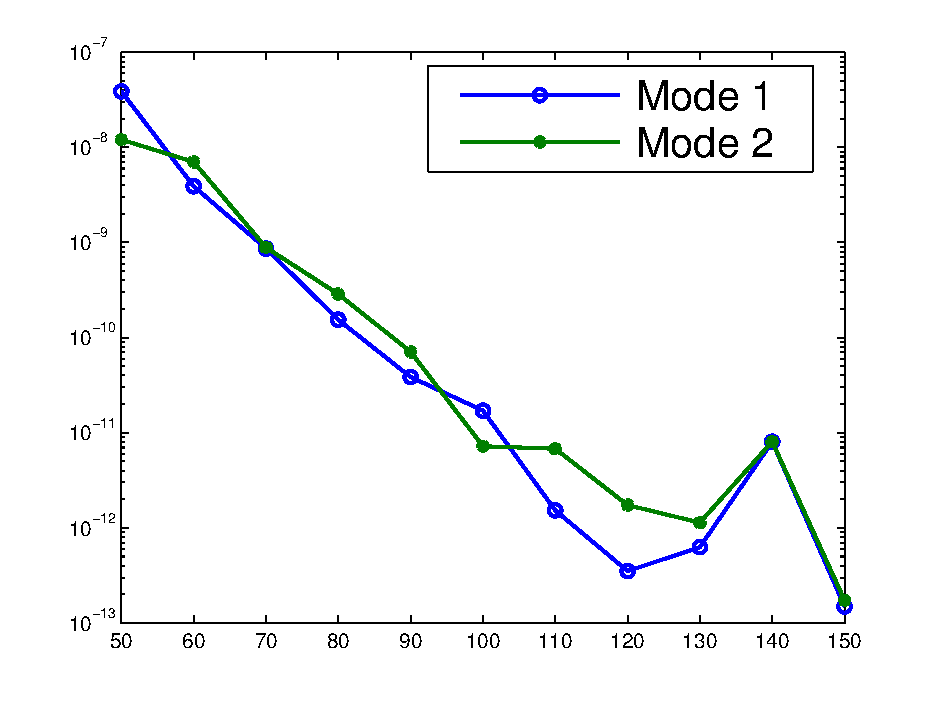
\includegraphics[height=0.74\textheight]{convergence3_cropped.pdf}
\end{center}
\vspace{-0.5em}
\begin{center}
\scriptsize Relative effective-index error versus points per hole. The
reference value uses 200 points on each hole boundary.
\end{center}
\end{frame}

%================================================================
\begin{frame}{Rectangular waveguide: relative field-error convergence}
\small
\begin{center}
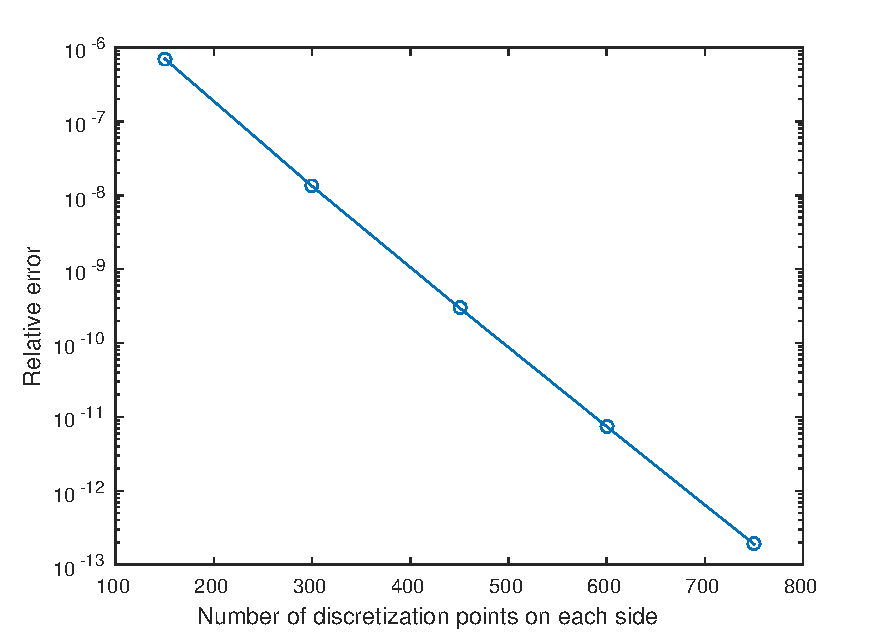
\includegraphics[height=0.72\textheight]{rectfig1_cropped.pdf}
\end{center}
\vspace{-0.5em}
\begin{center}
\footnotesize The vertical axis is relative field error (log scale); the
horizontal axis is the number of points on each side of the square.
\end{center}
\end{frame}

%================================================================
\begin{frame}{Rectangular waveguide: SKIE versus SREP singular values}
\small
\begin{center}
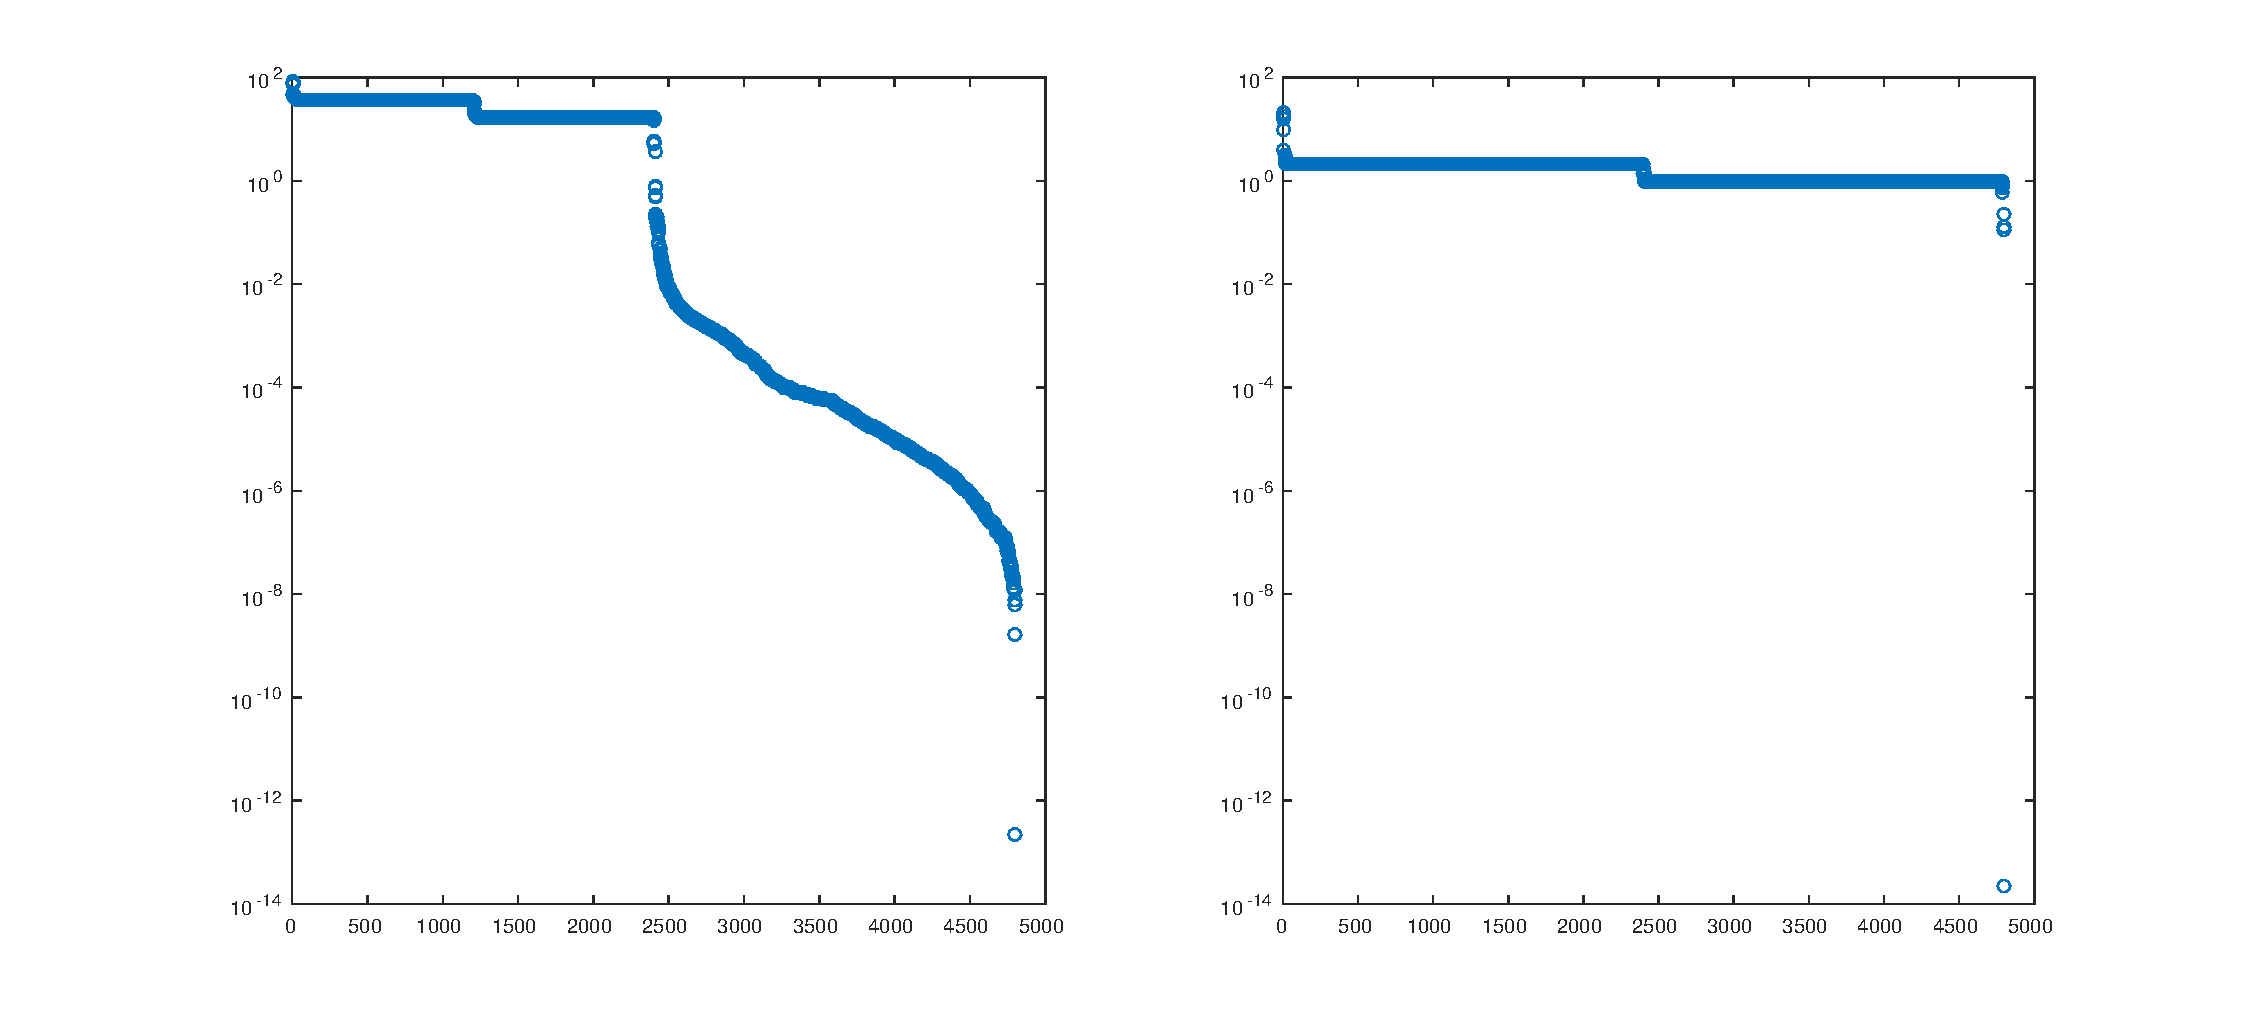
\includegraphics[height=0.72\textheight]{rectfig2_cropped.pdf}
\end{center}
\vspace{-0.5em}
\begin{center}
\footnotesize Left: single-layer representation (SREP). Right: SKIE. The
two near-null singular values in the SKIE plot correspond to the double mode.
\end{center}
\end{frame}

%================================================================
\begin{frame}{What the SKIE formulation provides}
\small
\begin{itemize}
  \item A two-dimensional second-kind integral equation formulation derived
  from the mode ansatz and the dual Muller representation.
  \item Unknown densities only on material interfaces, reducing the
  discretization dimension by one.
  \item High-order quadrature on smooth interfaces and corner-refined chunks
  for nonsmooth geometries.
  \item A scalar Muller root function for the nonlinear effective-index
  equation.
  \item Accurate propagation constants, including the small imaginary part
  associated with modal loss.
\end{itemize}
\end{frame}

%================================================================
\begin{frame}{References}
\scriptsize
\begin{itemize}
  \item J. Wang, J. Su, L. Greengard, S. Jiang, and S. Veerapaneni,
  ``Space-time adaptive methods for parabolic evolution equations,''
  arXiv:2511.18180 (2025).
  \item L. Greengard, S. Jiang, M. Rachh, and J. Wang, ``A new version of the
  adaptive fast Gauss transform for discrete and continuous sources,''
  \emph{SIAM Review}, 66(2) (2024).
  \item J. Lai and S. Jiang, ``Second kind integral equation formulation for the
  mode calculation of optical waveguides,'' \emph{Applied and Computational
  Harmonic Analysis}, 44(3) (2018), 645--664.
  \item D. E. Muller, ``A method for solving algebraic equations using an
  automatic computer,'' \emph{Mathematical Tables and Other Aids to
  Computation}, 10 (1956), 208--215.
\end{itemize}
\end{frame}

\end{document}
